\section{Introduction}

This note is intended to describe the design and implementation of the
pixel online software. The pixel online software is used for controlling and calibrating the CMS pixel
detector. In particular, it performs the following functions:
\begin{itemize}
\item Configure the detector
\item Perform online calibrations
%JMT: isn't this outside the scope of POS?
\item Analyze calibration data in online farm (CMSSW)
\item Monitor the detector during data taking
%\item Control the detector environment (DCS)
\end{itemize}

In Section~\ref{sect:overview} the main software components 
are introduced. Next the software organization is discussed.
In Section~\ref{sect:swcomponets} the different software components
are discussed in more detail. In Section~\ref{sect:calib} the
different calibrations are described. Other information about
pixel online software is available at the pixel online
software wiki pages~\cite{poswiki}.

\section{Pixel DAQ System}

The intention of this section it to give an overview of
the CMS pixel DAQ system. For more details the reader
can follow the references given in the text. But the
introduction given here should be sufficient to understand
the main goals of the pixel software.

\subsection{Overview of DAQ components}

The CMS pixel DAQ system consists of a number of 
components as illustrated in Fig.~\ref{fig:daqcomponents}.
This figure is specific to the FPix detector, but the
modification for the BPix are minor and not really 
relevant to the discussion here unless otherwise 
mentioned. Starting from the detector itself we have the the
Read Out Chip (ROC)~\cite{ROC} and the token bit manager 
(TBM)~\cite{TBM}. Some properties of the ROC are described 
below as needed to understand the calibrations. The
ROC reads out 4,160 pixels and the TBM coordinates
the communication with a group of 8 to 24 ROCs.
The TBM is electrically connected to the portcard via
extension cables $\approx 2$ feet in length.

The portcard receives and sends optical signals to the
FrontEnd Controller (FEC) and FrontEnd Driver (FED)
respectively. The FEC is used to program the TBM 
and ROCs and the data read out from the detector is
send to the FED to be digitized. The portcard is the
home of several discrete components. We have the 
Digital Optic Hybrid (DOH) that receives data from
the FEC and the Analog Optic Hybrid (AOH) that 
transmits data to the FED. On the portcard we
have in addition the (t)PLL, Delay25, and gatekeeper
chips. 

Of particular interest is the Delay25 chip. The communication
to the portcard via the DOH is done at 40MHz on a serial
line. We have a clock line and the data line (and return clock
and return data). In order to have this communication
working the timing between the clock and data lines must
be right. The purpose of the Delay25 chip is to adjust
delays to make this communication work. The setting of the
parameters on the Delay25 chip as well as the other components
on the portcard is done using the I2C protocol from the
CCU. The CCU is again controlled from a Tracker FEC (TkFEC).

\begin{figure}[h]
\begin{center}
 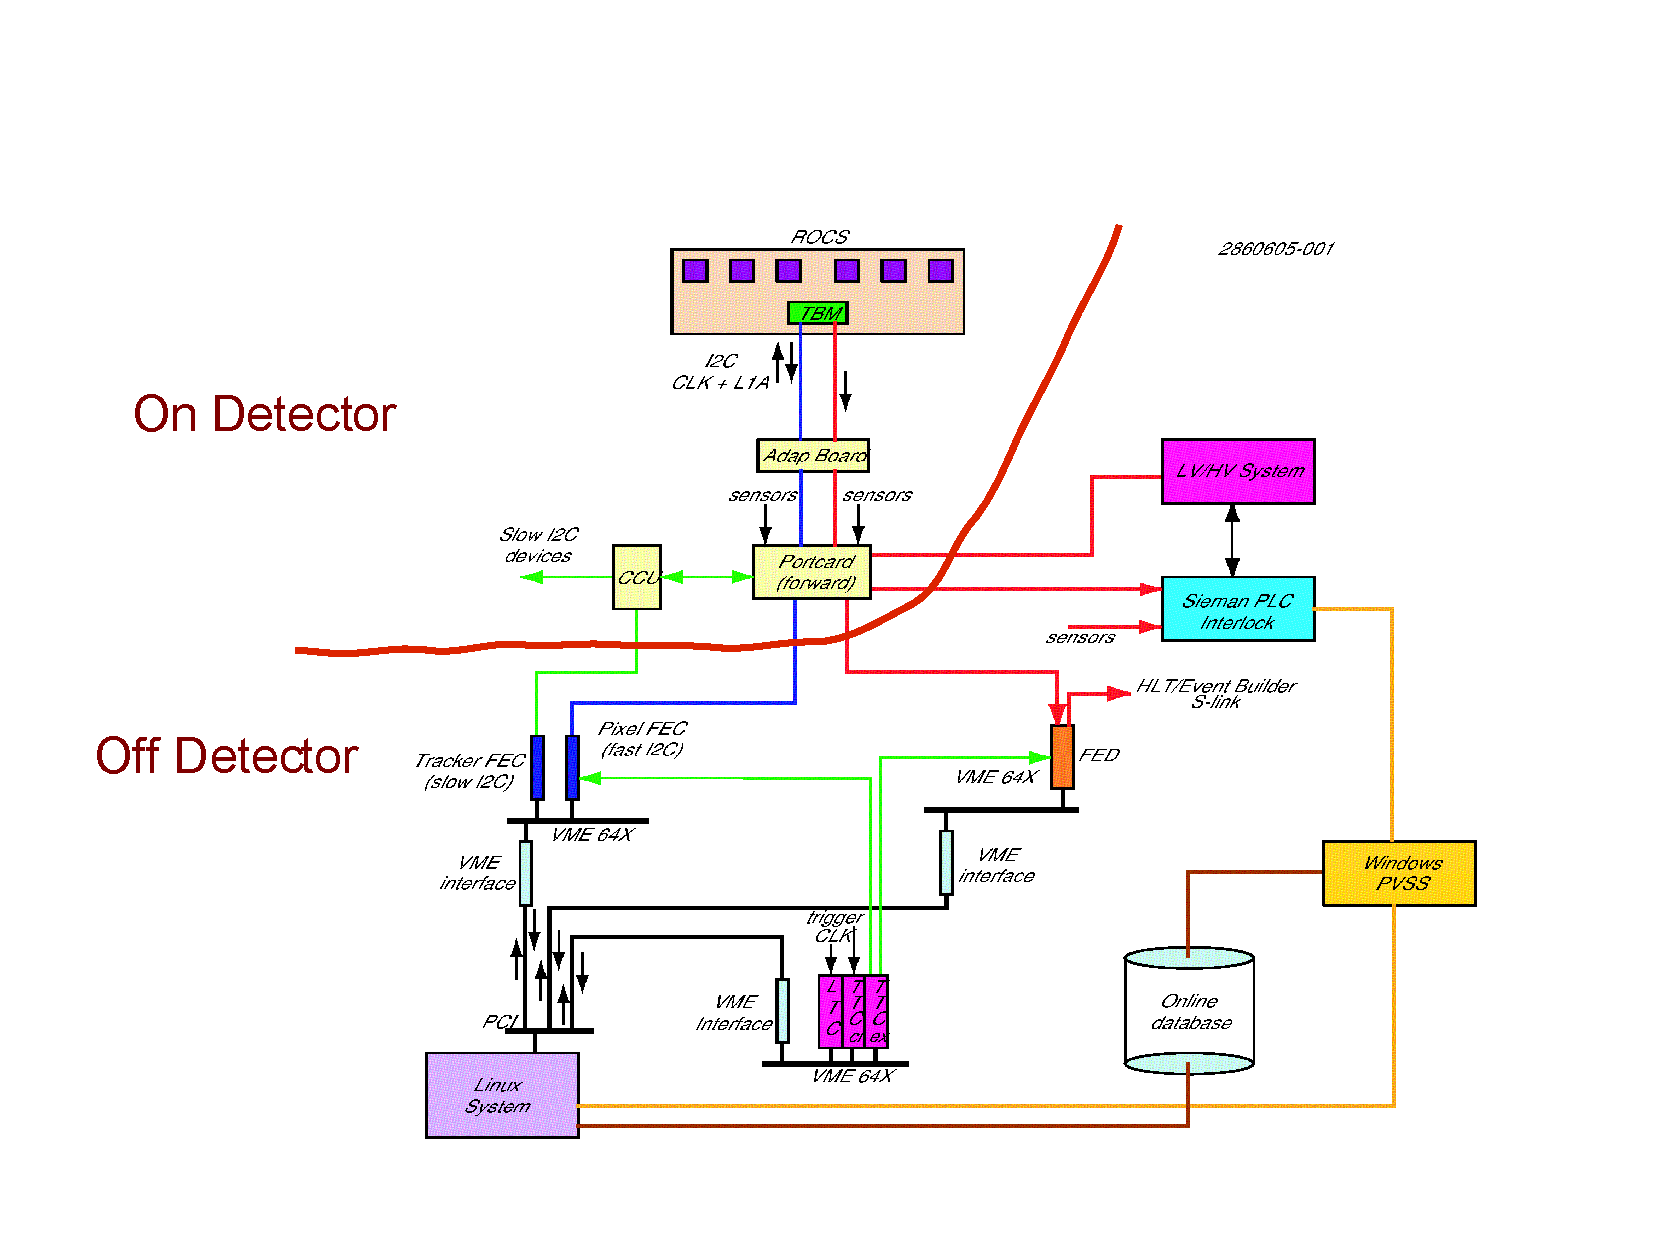
\includegraphics[width=0.99\textwidth]{2860506-001}
\end{center}
\caption{The main components in the CMS pixel DAQ system. }
\label{fig:daqcomponents}
\end{figure}

\clearpage

\subsubsection{The Read Out Chip}

Each Read Out Chip (ROC)~\cite{ROC}, ilustrated in Fig.~\ref{fig:ROC} collates data from 52 $\times$ 80 = 4,160 pixels 
and contains about 1.3 million transistors in all.
It amplifies and zero suppresses data using 4 trim bits
that specify a threshold for every pixel. The chip buffers hit data
until the trigger decision arrives. It is developed at PSI and manufactured by IBM.

\begin{figure}[h]
\begin{center}
 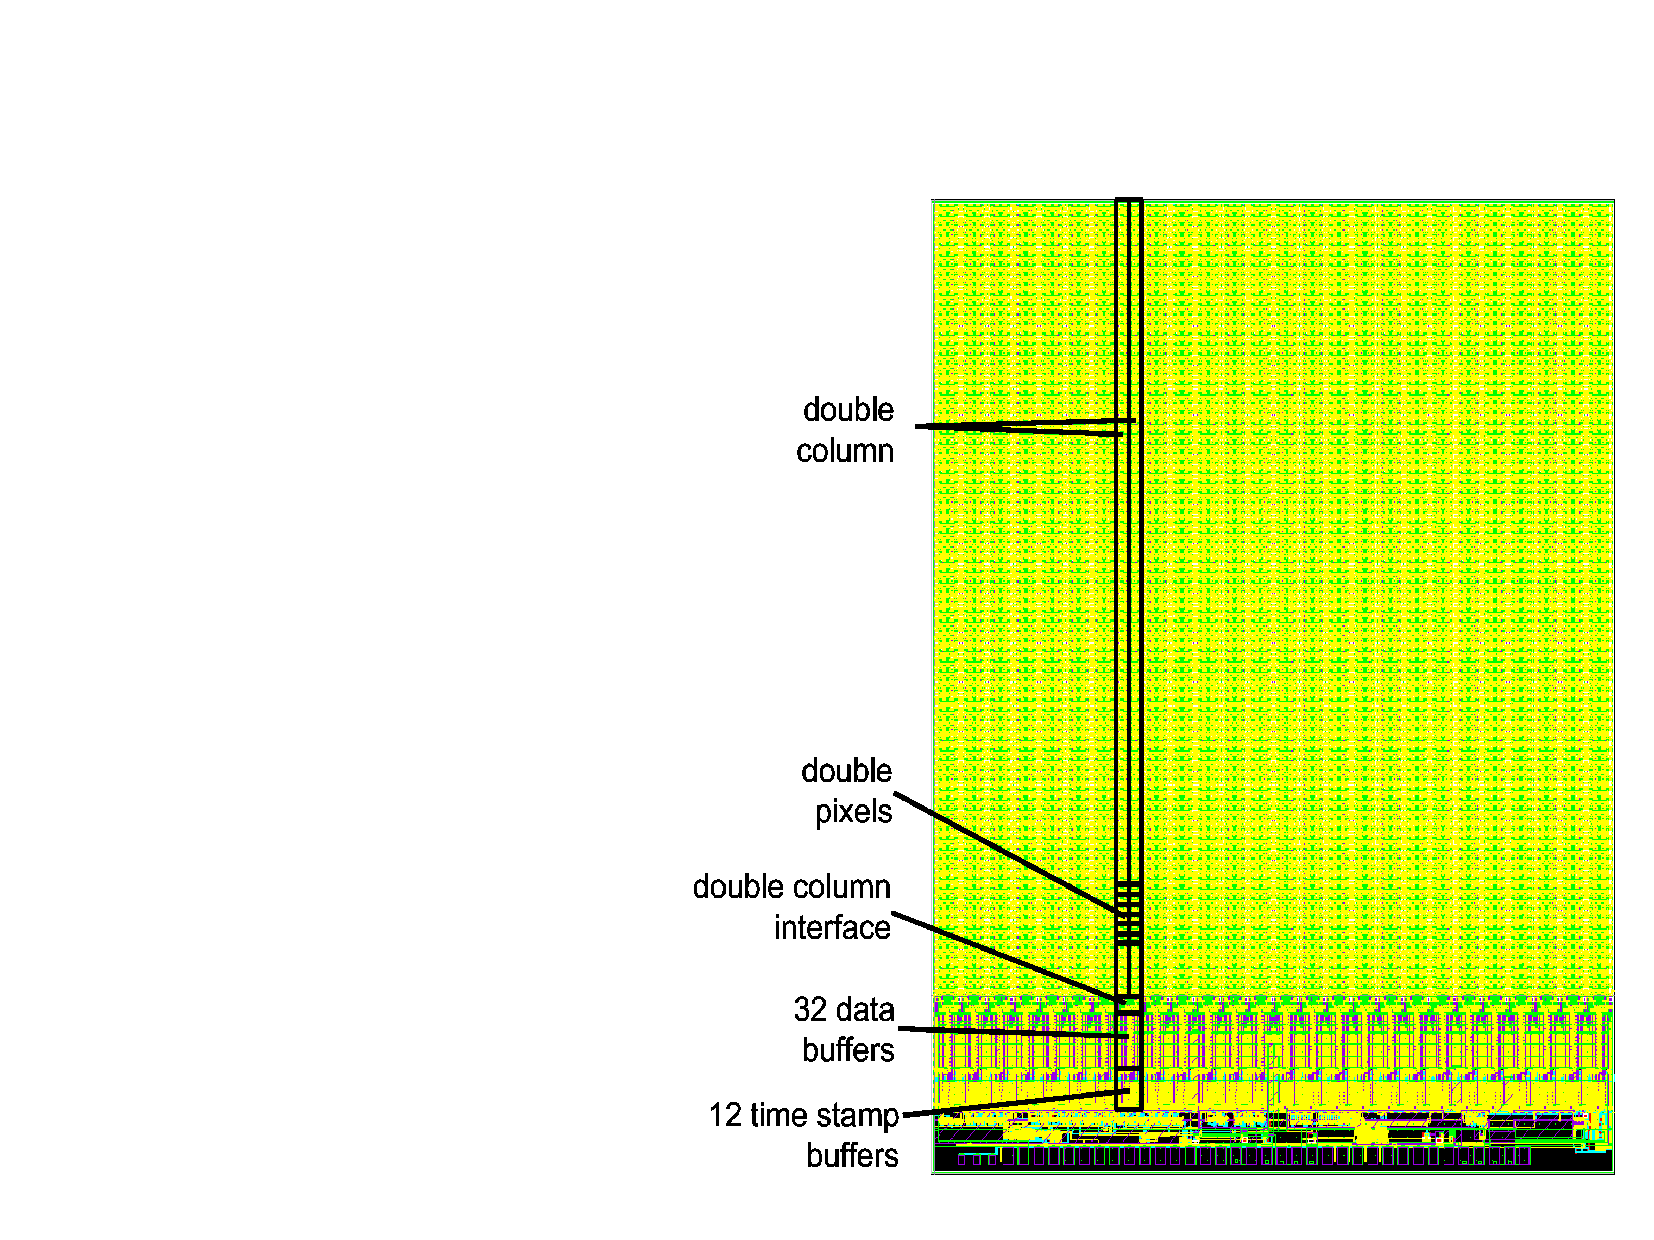
\includegraphics[width=0.45\textwidth]{ROC.pdf}
\end{center}
\caption{The Read Out Chip of the CMS Pixel Detector.}
\label{fig:ROC}
\end{figure}

\clearpage

\subsubsection{The Token Bit Manager}

A Token Bit Manager (TBM) controls groups of 8 to 24 ROCs.
It distributes the clock and trigger signals.
It serializes analog readout using a token bit 
passed from ROC to ROC. It is physically mounted next to the ROCs.
The TBM is developed at Rutgers.

\begin{figure}[h]
\begin{center}
 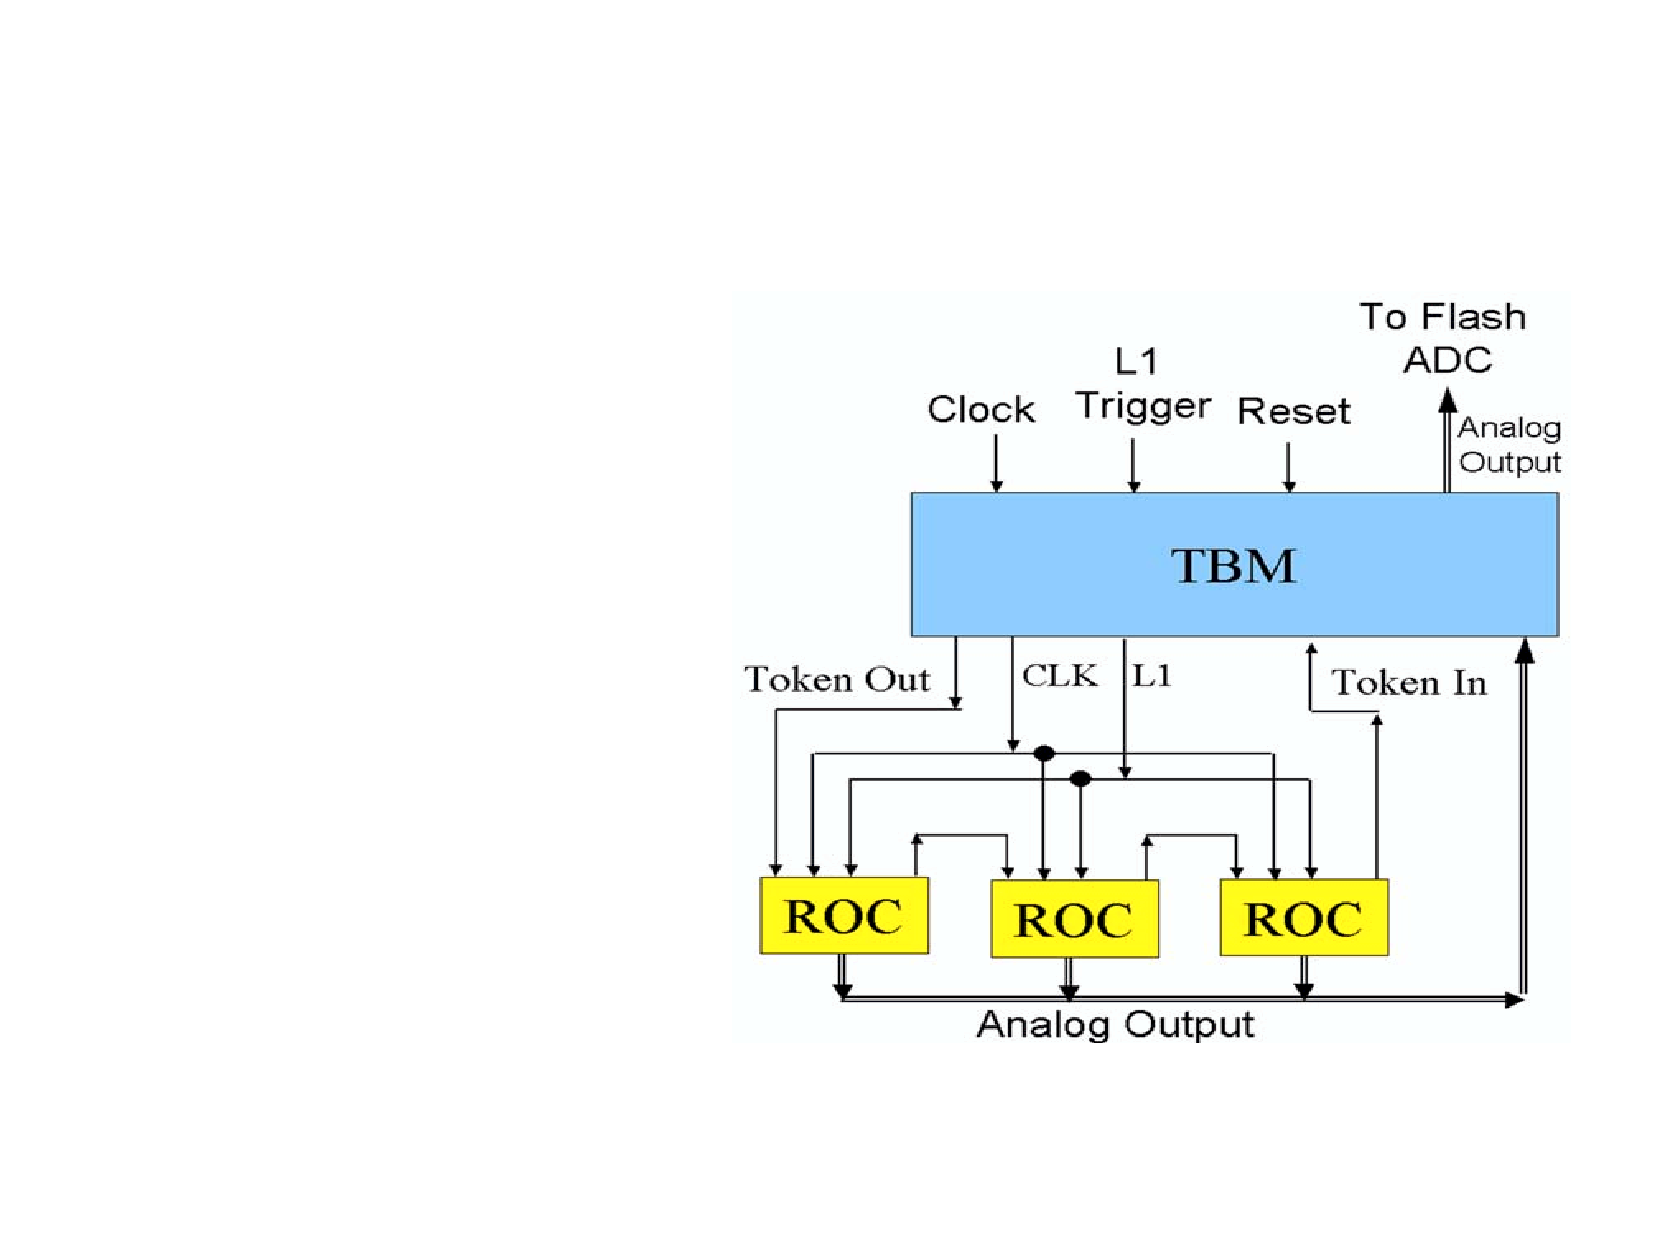
\includegraphics[width=0.45\textwidth]{TBM.pdf}
\end{center}
\caption{A schematic of how the Token Bit Manager reads out data from the ROCs.}
\label{fig:TBM}
\end{figure}

\clearpage

\subsubsection{The Pixel FED}

The Pixel Front End Driver (FED) is a VME module
with 36 optical inputs. It sits in the counting room and receives the analog output
of the ROCs via an optical fiber from the center of the CMS detector.
In order for the FED to decode and digitize this data, it has to have address levels 
well calibrated, and this is one of the several tasks performed by the Pixel Online Software.
Internal timings of the FED also have to be calibrated within errors of a few nanoseconds,
and this is also accomplished using the POS. The output of the FED
is dispatched, in a binary format readable to the entire CMS experiment, via an S-Link.

\begin{figure}[h]
\begin{center}
 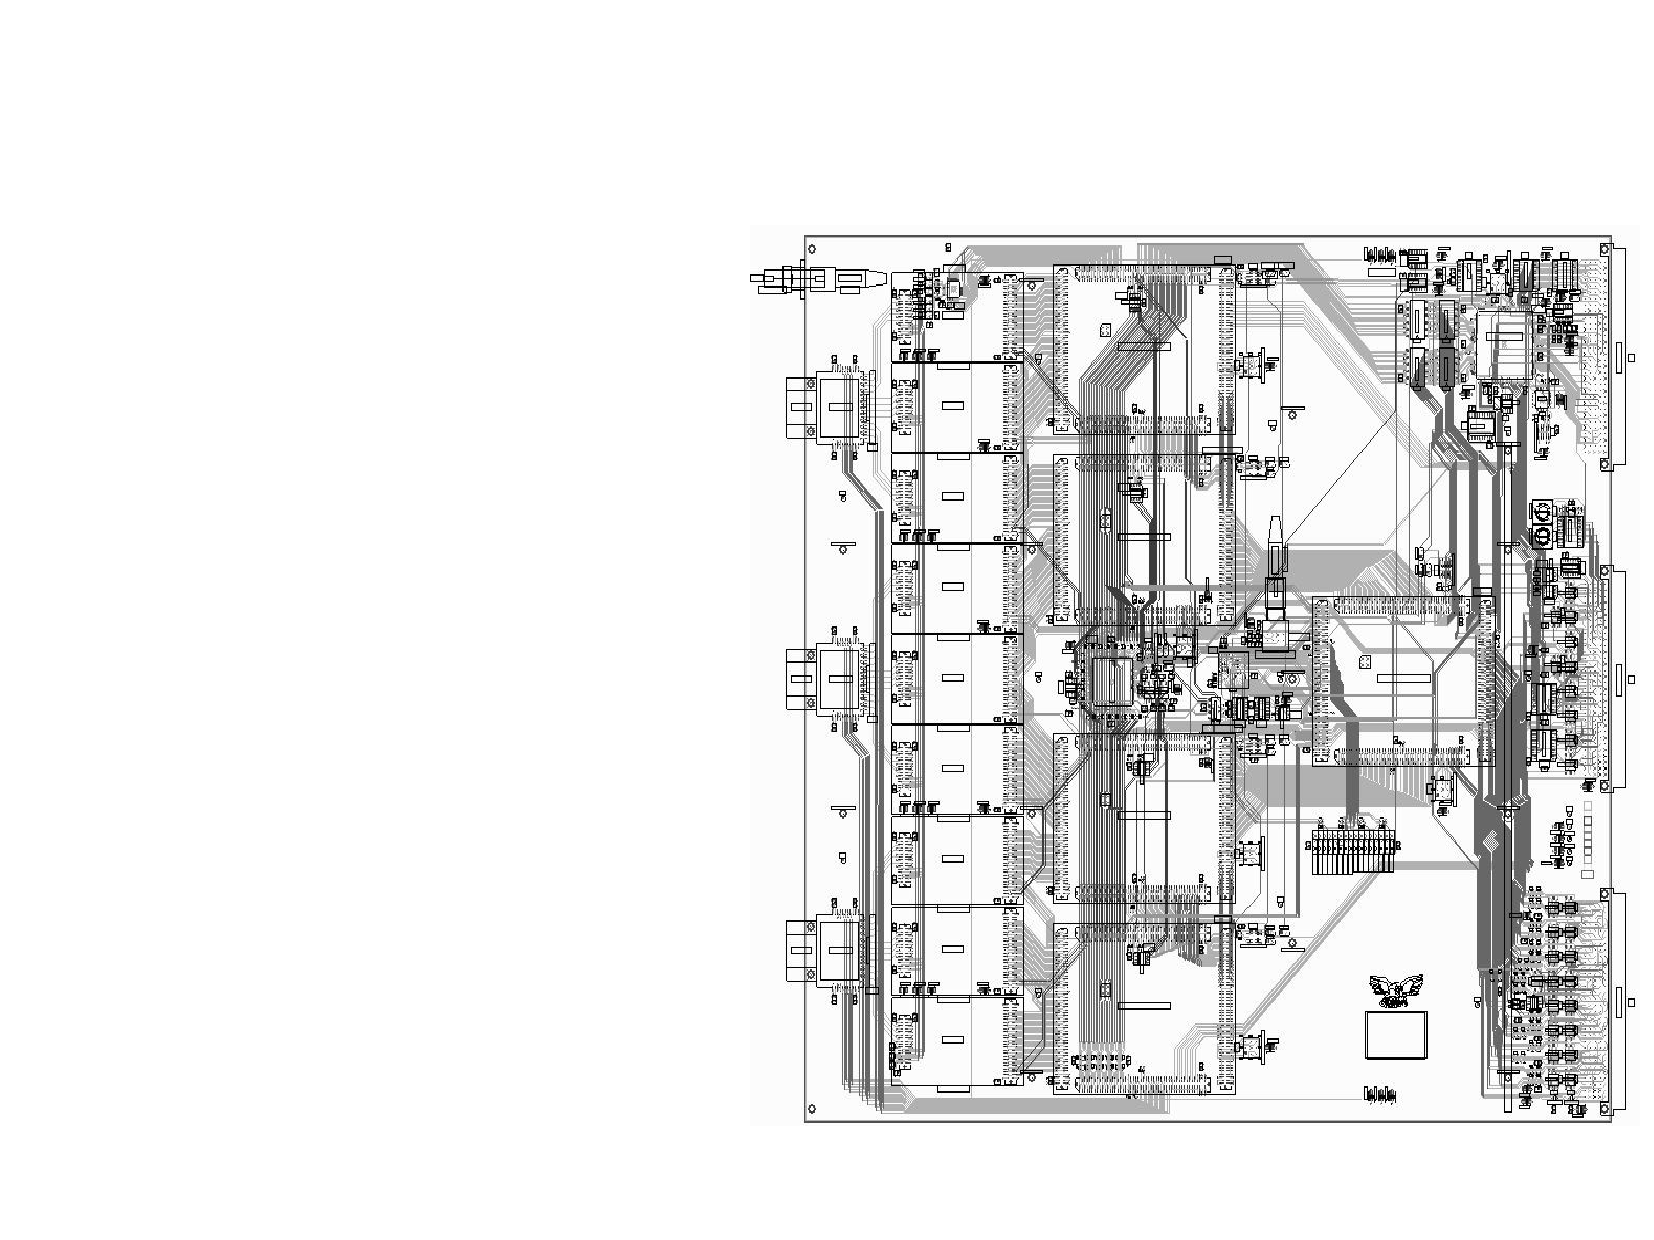
\includegraphics[width=0.45\textwidth]{pFED.pdf}
\end{center}
\caption{A schematic of the pixel FED.}
\label{fig:pFED}
\end{figure}

\clearpage

\subsubsection{The Pixel FEC}

The Pixel Front End Controller (FEC) sends triggers, clocks 
and programming data to the ROCs. For the pixel detector, 
we use a one-way `fast' I2C protocol to send this data.
We need to send 1 byte of data per pixel, or 66 MB of data
for the entire detector. For this, we use a 40 MHz serial line, 
and this calls for timing calibrations in order to enable downloads.

\begin{figure}[h]
\begin{center}
 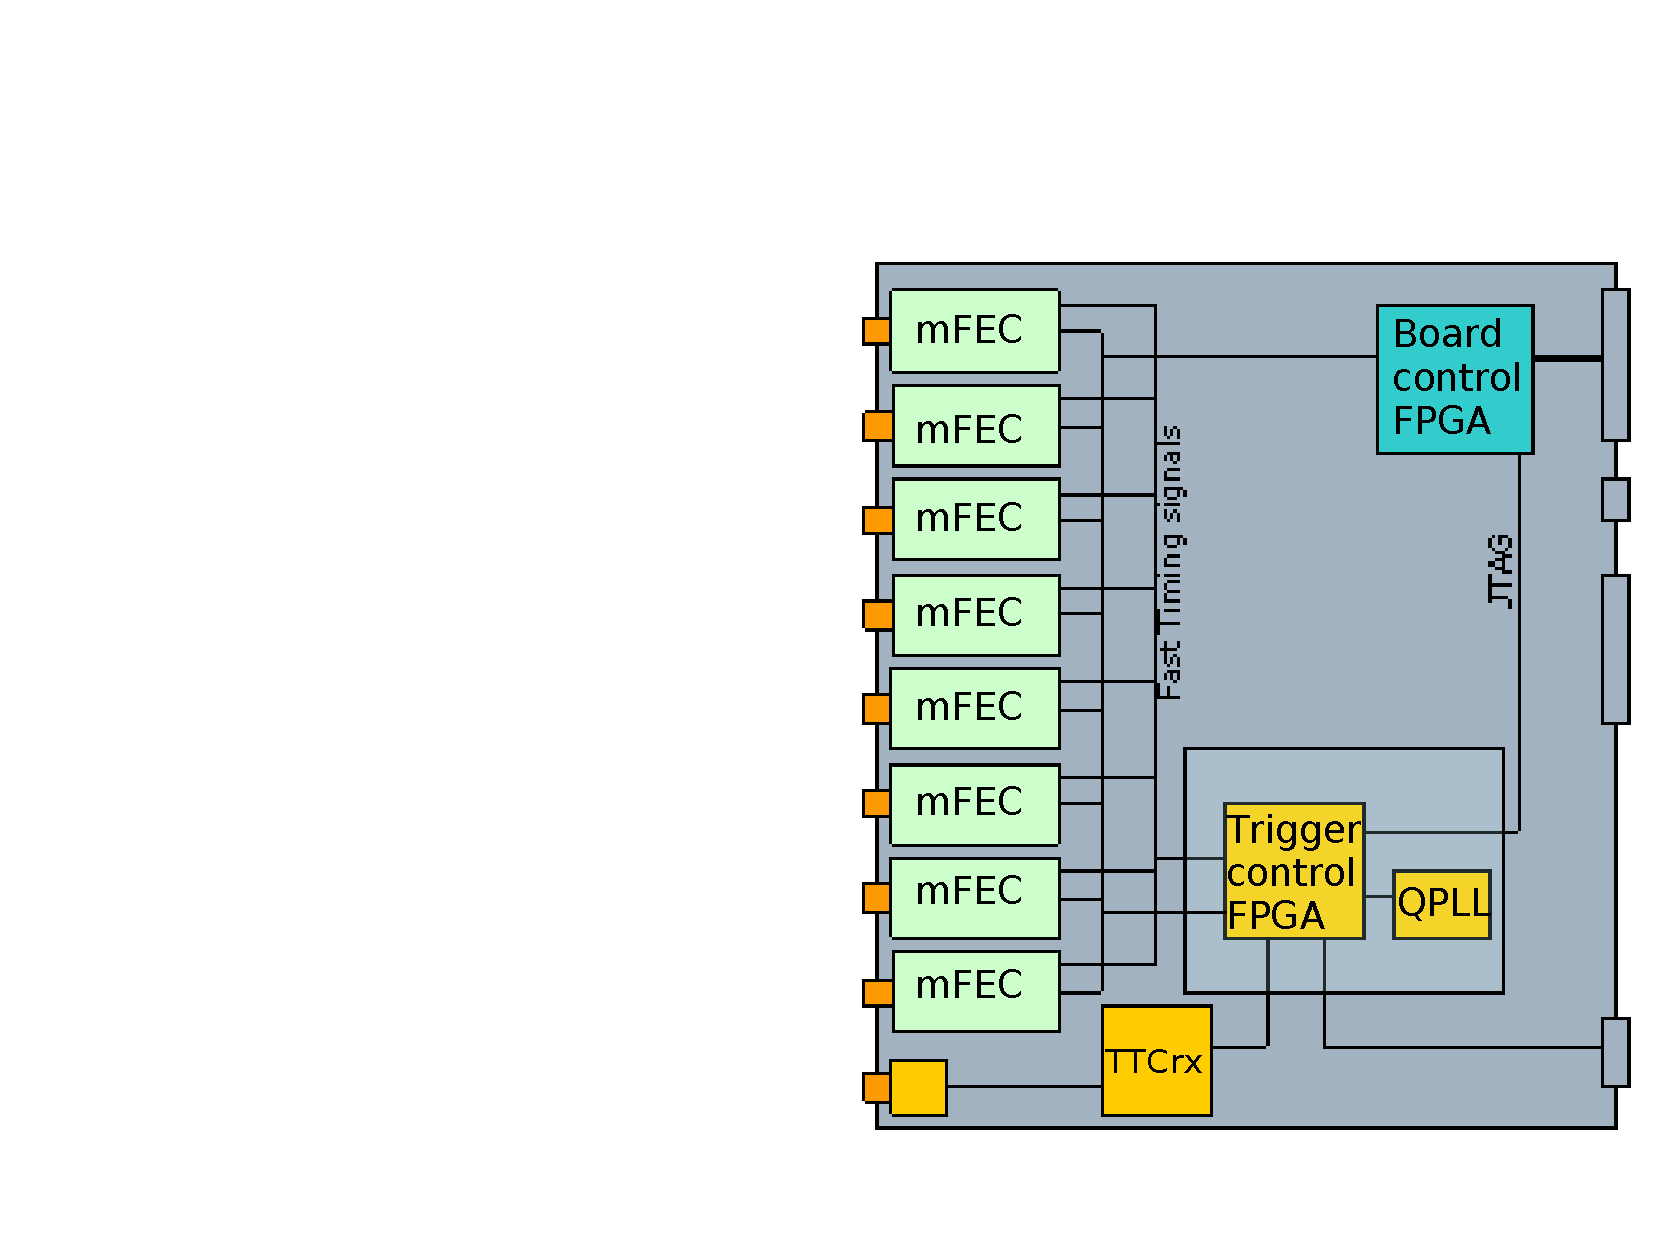
\includegraphics[width=0.45\textwidth]{pFEC.pdf}
\end{center}
\caption{A schematic of the pixel FEC.}
\label{fig:pFEC}
\end{figure}

\clearpage

\subsection{Installation at P5}

Table~\ref{tab:P5PCs} lists the online PCs that we have at P5
for pixel online software.

\begin{table}
\centering
\caption{Pixel online PCs at P5}
\label{tab:P5PCs}
\resizebox{\textwidth}{!}{
\begin{tabular}{lcccccccc}
\hline
\hline
Slot in rack & Node name     & Front & Label & Size & Function        & Comments     & OS \\ 
\hline
          -  & vmepcs2b18-17 & Pixel & -  & ?U      &  Histoviewer    &              & SLC4 \\
          19 & vmepcs2b18-16 & Pixel & 1/10  & 1U   &  VME/S1G01i     & BPix FECs    & SLC4 \\
          17 & vmepcs2b18-15 & Pixel & 10/10 & 1U   &  VME/S1G01e     & FPix FECs    & SLC4 \\
          16 & vmepcs2b18-14 & Pixel & 9/10  & 1U   &  VME/S1G04e     & BPix FEDs do & SLC4 \\
      14/15  & vmepcs2b18-13 & Pixel & 8/10  & 2U   &  VME/S1G04i     & BPix FEDs up & SLC4 \\
          13 & vmepcs2b18-12 & Pixel & 7/10  & 1U   &  VME/S1G03i     & FPix FEDs    & SLC4 \\
          12 & vmepcs2b18-11 & Pixel & 6/10  & 1U   &  PixelSuperFPix & FPix Supv.   & SLC4 \\
          11 & vmepcs2b18-10 & Pixel & 5/10  & 1U   &  PixelSuperBPix & BPix Supv.   & SLC4 \\
          10 & vmepcs2b18-09 & Pixel & 4/10  & 1U   &  DCS            & Fpix daq     & Win \\
           9 & vmepcs2b18-08 & Pixel & 3/10  & 1U   &  DCS/Siemens    &              & Win \\
           8 & vmepcs2b18-07 & Pixel & 2/10  & 1U   &  DCS/CAEN       &              & Win \\
             & vmepcs2b16-10 &       &       &      &  TTC+LTC Supv.  & TTC+LTC      & SLC4 \\
             &  cmsrc-pixel  &       &       &      &  L1 FM          & Pixel FM     & SLC4 \\
             &fmmpc-s1d12-08 &       &       &      &  FMM PC         & FMM PC       & SLC4 \\
             &  cmspsx       &       &       &      &  PSX server     & PSX server   & SLC4 \\
             &  srv-c2c02-05 &       &       &      &  DB server      &              & SLC4 \\
             &  srv-c2c02-06 &       &       &      &  DB server      &              & SLC4 \\
\hline
\hline
\end{tabular}
}
\end{table}

\begin{small}
\begin{table}
\centering
\caption{FED connections for FPIX}
\label{tab:FpixFED}
\resizebox{\textwidth}{!}{
\begin{tabular}{llcccclc}
\hline
\hline
Rack   & Crate   & Slot & VME addr.  & Channels & FED id & Name(Official) & Name(Construction) \\
\hline
S1G03  & upper   & 6    & 0x13000000 &  13-24   & 33     & BpO\_D(1,2)\_BLD(1,2,3)    & HC+Z1 1.1 2.1\\
S1G03  & upper   & 6    & 0x13000000 &  1-12    & 33     & BpO\_D(1,2)\_BLD(4,5,6)    & HC+Z1 1.2 2.2\\
S1G03  & upper   & 7    & 0x14000000 &  13-24   & 34     & Bp0\_D(1,2)\_BLD(7,8,9)    & HC+Z1 1.3 2.3\\
S1G03  & upper   & 7    & 0x14000000 &  1-12    & 34     & Bp0\_D(1,2)\_BLD(10,11,12) & HC+Z1 1.4 2.4\\
\hline
S1G03  & upper   & 5    & 0x12000000 &  1-12    & 32     & BpI\_D(1,2)\_BLD(1,2,3)    & HC+Z2 1.4 2.4\\
S1G03  & upper   & 5    & 0x12000000 &  13-24   & 32     & BpI\_D(1,2)\_BLD(4,5,6)    & HC+Z2 1.3 2.3\\
S1G03  & upper   & 8    & 0x15000000 &  1-12    & 35     & BpI\_D(1,2)\_BLD(7,8,9)    & HC+Z2 1.2 2.2\\
S1G03  & upper   & 8    & 0x15000000 &  13-24   & 35     & BpI\_D(1,2)\_BLD(10,11,12) & HC+Z2 1.1 2.1\\
\hline
S1G03  & upper   & 11   & 0x17000000 &  13-24   & 37     & BmI\_D(1,2)\_BLD(1,2,3)    & HC-Z1 1.1 2.1\\
S1G03  & upper   & 11   & 0x17000000 &  1-12    & 37     & BmI\_D(1,2)\_BLD(4,5,6)    & HC-Z1 1.2 2.2\\
S1G03  & upper   & 12   & 0x18000000 &  13-24   & 38     & BmI\_D(1,2)\_BLD(7,8,9)    & HC-Z1 1.3 2.3\\
S1G03  & upper   & 12   & 0x18000000 &  1-12    & 38     & BmI\_D(1,2)\_BLD(10,11,12) & HC-Z1 1.4 2.4\\
\hline
S1G03  & upper   & 10   & 0x16000000 &  1-12    & 36     & BmO\_D(1,2)\_BLD(1,2,3)    & HC-Z2 1.4 2.4\\
S1G03  & upper   & 10   & 0x16000000 &  13-24   & 36     & BmO\_D(1,2)\_BLD(4,5,6)    & HC-Z2 1.3 2.3\\
S1G03  & upper   & 13   & 0x19000000 &  1-12    & 39     & BmO\_D(1,2)\_BLD(7,8,9)    & HC-Z2 1.2 2.2\\
S1G03  & upper   & 13   & 0x19000000 &  13-24   & 39     & BmO\_D(1,2)\_BLD(10,11,12) & HC-Z2 1.1 2.1\\
\hline
\hline
\end{tabular}
}
\end{table}
\end{small}

\begin{small}
\begin{table}
\centering
\caption{FEC connections for FPIX}
\label{tab:FpixFEC}
\resizebox{\textwidth}{!}{
\begin{tabular}{llllclc}
\hline
\hline
Rack   & Crate   & Slot & VME addr. & mFEC & Name(Official) & Name(Construction) \\
\hline
S1G01  & middle  & 5    & 0x28000000 & 3    & BpO\_D(1,2)\_BLD(1,2,3)    & HC+Z1 1.1 2.1\\
S1G01  & middle  & 5    & 0x28000000 & 4    & BpO\_D(1,2)\_BLD(4,5,6)    & HC+Z1 1.2 2.2\\
S1G01  & middle  & 5    & 0x28000000 & 5    & Bp0\_D(1,2)\_BLD(7,8,9)    & HC+Z1 1.3 2.3\\
S1G01  & middle  & 5    & 0x28000000 & 6    & Bp0\_D(1,2)\_BLD(10,11,12) & HC+Z1 1.4 2.4\\
\hline
S1G01  & middle  & 5    & 0x28000000 & 8    & BpI\_D(1,2)\_BLD(1,2,3)    & HC+Z2 1.4 2.4\\
S1G01  & middle  & 5    & 0x28000000 & 7    & BpI\_D(1,2)\_BLD(4,5,6)    & HC+Z2 1.3 2.3\\
S1G01  & middle  & 5    & 0x28000000 & 2    & BpI\_D(1,2)\_BLD(7,8,9)    & HC+Z2 1.2 2.2\\
S1G01  & middle  & 5    & 0x28000000 & 1    & BpI\_D(1,2)\_BLD(10,11,12) & HC+Z2 1.1 2.1\\
\hline
S1G01  & middle  & 10   & 0x50000000 & 3    & BmI\_D(1,2)\_BLD(1,2,3)    & HC-Z1 1.1 2.1\\
S1G01  & middle  & 10   & 0x50000000 & 4    & BmI\_D(1,2)\_BLD(4,5,6)    & HC-Z1 1.2 2.2\\
S1G01  & middle  & 10   & 0x50000000 & 5    & BmI\_D(1,2)\_BLD(7,8,9)    & HC-Z1 1.3 2.3\\
S1G01  & middle  & 10   & 0x50000000 & 6    & BmI\_D(1,2)\_BLD(10,11,12) & HC-Z1 1.4 2.4\\
\hline
S1G01  & middle  & 10   & 0x50000000 & 8    & BmO\_D(1,2)\_BLD(1,2,3)    & HC-Z2 1.4 2.4\\
S1G01  & middle  & 10   & 0x50000000 & 7    & BmO\_D(1,2)\_BLD(4,5,6)    & HC-Z2 1.3 2.3\\
S1G01  & middle  & 10   & 0x50000000 & 2    & BmO\_D(1,2)\_BLD(7,8,9)    & HC-Z2 1.2 2.2\\
S1G01  & middle  & 10   & 0x50000000 & 1    & BmO\_D(1,2)\_BLD(10,11,12) & HC-Z2 1.1 2.1\\
\hline
\hline
\end{tabular}
}
\end{table}
\end{small}

\begin{small}
\begin{table}
\centering
\caption{CCU connections for FPIX}
\label{tab:FpixCCU}
\begin{tabular}{llcccc}
\hline
\hline
Rack   & Crate   & Slot & mFEC & Name(Official) & Name(Construction) \\
\hline
S1G01  &  middle & 18   &  8   & BpI            & HC+Z2 \\
S1G01  &  middle & 18   &  7   & BpO            & HC+Z1 \\
S1G01  &  middle & 18   &  6   & Bm0            & HC-Z2 \\
S1G01  &  middle & 18   &  5   & BmI            & HC-Z1 \\
\hline
\hline
\end{tabular}
\end{table}
\end{small}


\section{Online Software Overview} 
\label{sect:overview}

The pixel online software is based on the xdaq toolkit and is
built from a number of different components (applications). The
different xdaq based components are shown in green in 
Fig.~\ref{fig:components}. The top level application is the 
PixelSupervisor. This application is responsible for the overall
coordination of the pixel DAQ. The PixelSupervisor talks to the
supervisors that directly control the hardware. For example 
we have the PixelFECSupervisor that provides the interface to the
pixel FECs. Similarly the PixelFEDSupervisor controls FEDs. 
In production at P5, there are multiple instances of the PixelFECSupervisor and
PixelFEDSupervisor; one per VME crate.\footnote{The strip tracker
uses a design where there is one supervisor per VME board.}

The PixelTKFECSupervisor controls the tracker FEC hardware. The
pixel system uses the tracker FEC hardware slow I2C to
initialize the fast I2C used for the download of most 
configuration data.

The PixelTTCSupervisor controls the pixel TTC module used for trigger
and timing. Among other things the TTC module is used during
calibrations to generate triggers. In modern releases of the software,
the PixelTTCSupervisor has been deprecated in favor of the
TTCciControl, which is a standard package maintained by the TTC group.

The PixelLTCSupervisor is used for the local trigger control.

The various supervisors run as indepdendent processes, or even on
different computers. Therefore, in order to communicate with each
other they must exchange messages on the network. This is done using
the SOAP protocol.

The Level 1 function manager (L1FM or FM) for the pixels is the
interface the pixel system has to the global run control (RCMS for
Run Control and Monitoring System). The FM is a java application.
It responds to requests from RCMS to change states in the 
state diagram that describe the state of the DAQ system. This
state diagram is shown in Fig.~\ref{fig:l1fm}.  The pixel
FM is a relatively thin layer that basically just passes the state
changes on to the PixelSupervisor. 

\begin{figure}
\begin{center}
 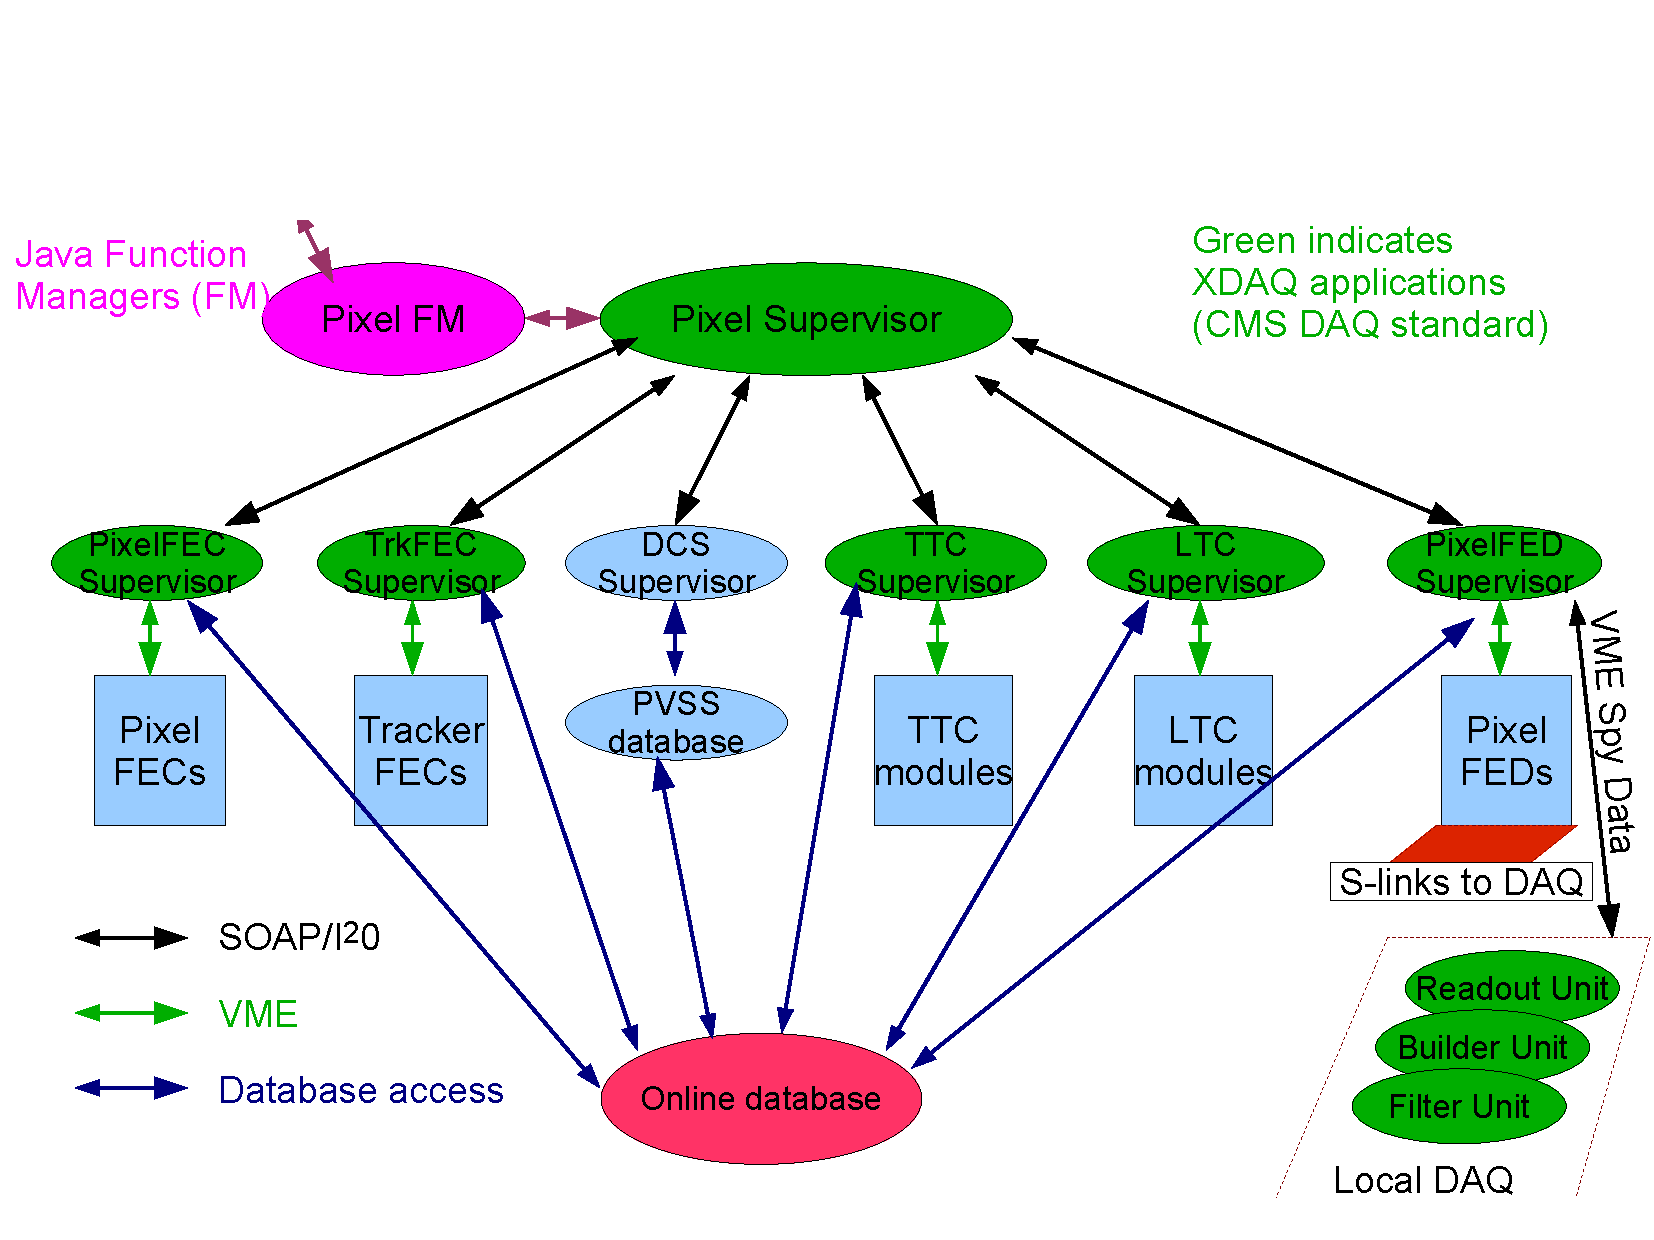
\includegraphics[width=0.99\textwidth]{POScomponents.pdf}
\end{center}
\caption{The different applications that compose the Pixel Online Software.}
\label{fig:components}
\end{figure}

\section{Package structure} \label{sect:swcomponets}

In the pixel online software the code is distributed
among a number of packages. These packages are listed
here.
\begin{itemize}
\item PixelCalibrations
%\item PixelCalibrationInterface
\item CalibFormats/SiPixelObjects
\item PixelConfigDBInterface
%\item PixelDCSSupervisor
\item PixelDCSInterface
\item PixelFECInterface
\item PixelFECSupervisor
\item PixelFEDInterface
\item PixelFEDSupervisor
\item PixelFunctionManager
\item PixelLTCSupervisor
\item PixelSupervisor
\item PixelTKFECSupervisor
\item PixelTTCSupervisor\footnote{In use through tag {\tt POS\_3\_1\_2}; deprecated starting in {\tt POS\_3\_2\_0}.}
\item PixelUtilities
\end{itemize}
The package dependency tree is shown in Fig~\ref{fig:dependencies}.
The supervisor applications are at the top and depend on the 
packages below. We should make sure that the dependencies
form a tree and not contain loops. (If it seems necessary
to create a loop the solution is almost always to separate
out some piece of code into a separate package.)


\begin{figure}
\begin{center}
 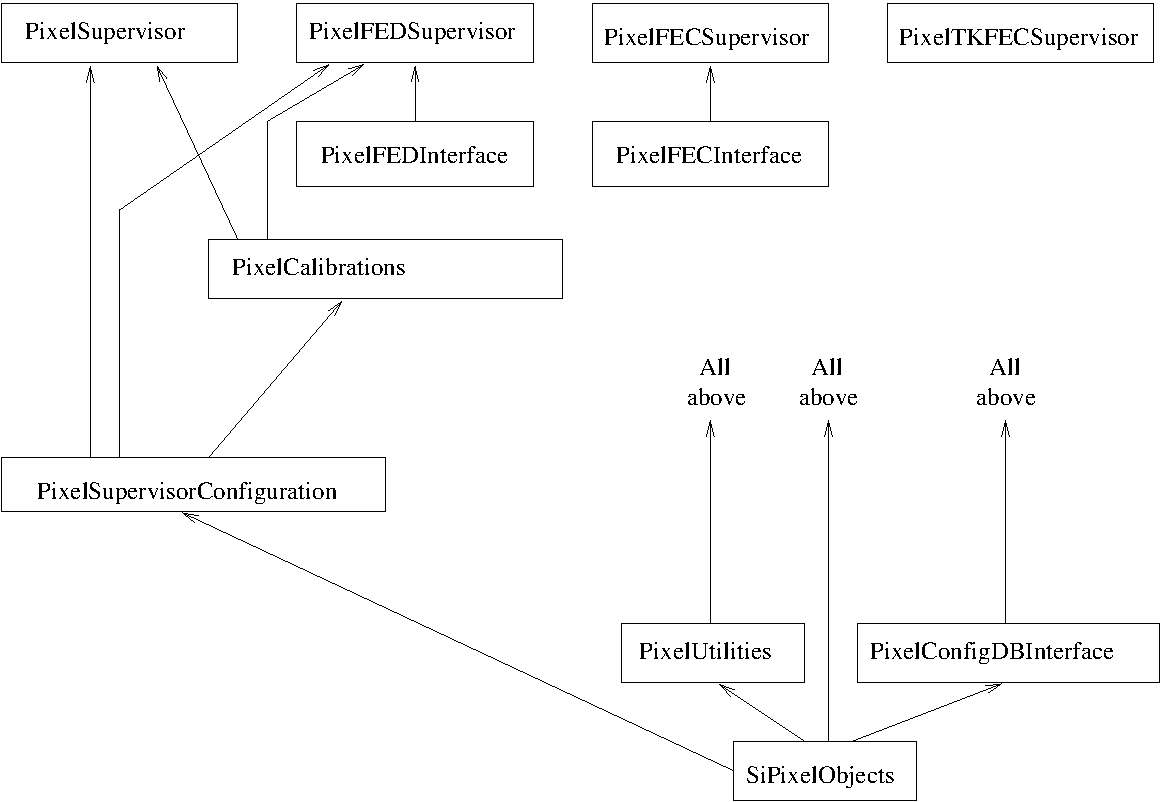
\includegraphics[width=0.99\textwidth]{package_dep.pdf}
\end{center}
\caption{The dependencies among the packages are indicated here.
At top are the supervisor applications. }
\label{fig:dependencies}
\end{figure}



\subsection{Pixel Function Manager}
\label{sec:l1fm}
The pixel function manager (the Level 1 Function Manager) acts as an interface between
run control (the level 0 function manager) and the pixel
online software. The pixel function manager is a java
application. It implements the state machine of 
CMS~\cite{statemachine}. The function manager interacts
with the PixelSupervisor to carry out the 
different tasks needed in state transitions of the
run control.

\begin{figure}
\begin{center}
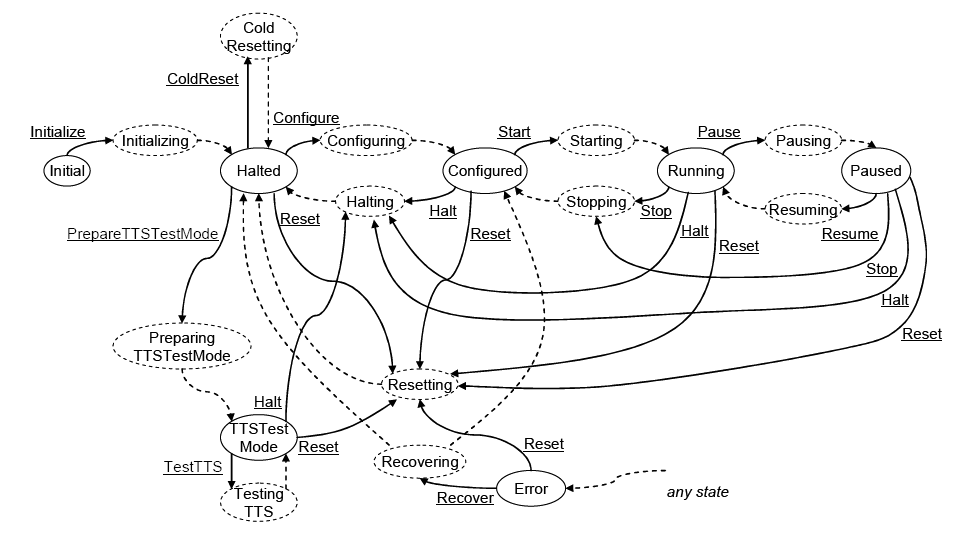
\includegraphics[width=0.99\textwidth]{l1fm_states.png}
\end{center}
\caption{The CMS finite state machine definition. Figure taken from Ref.~\cite{statemachine}.}
\label{fig:l1fm}
\end{figure}

\subsubsection{FSM Implementation Status}
The CMS run control finite state machine (FSM) is shown in
Fig.~\ref{fig:l1fm}. This model is implemented in the the pixel
function manager, and also in the PixelSupervisor. The other
Supervisors implement portions of this model as required. At the
moment, the FSM depicted in the figure is completely implemented in
the PixelSupervisor, with the exception of the ``Reset'' transition
and its accompanying ``Resetting'' state. The PixelSupervisor does
include transitions from any state into the ''Error'' state, and then
allows a ``Recover'' transition that returns the FSM to the ``Halted''
state.

\subsubsection{Control of the L1FM}

During global running, the L1FM is driven by the L0FM, which is
operated by central DAQ. The pixel user should not intervene via the
L1FM GUI, except to check its status.

During local running, the L1FM must be created via its GUI. State
transitions of the FSM can then be driven via the L1FM GUI. In
general, we drive the ``Initialize'' state transition via the GUI,
then drive subsequent state transitions directly from the
PixelSupervisor. However, in principle all transitions can be
initiated from the L1FM GUI.\footnote{In practice, this is only useful for simple tests of the L1FM to PixelSupervisor communication.}

\subsubsection{Outline of L1FM implementation}

The L1FM is created using the Create button in RCMS. This calls the
method of {\tt PixelFunctionManager.java} called {\tt
createAction()}.

After creation, transitions of the FM FSM are handled
by methods in {\tt PixelEventHandler.java}. Which method is triggered
depends on the transition, as defined by a table near the top of this
class. The names are fairly logical (for example, ``Initialize''
corresponds to the {\tt initAction} method and ``Configure''
corresponds to the {\tt configureAction} method). Inside each {\tt
fooAction} method are two blocks: one to handle objects of type {\tt
StateEnteredEvent} and one to handle objects of type {\tt
StateNotification}. 

When an FSM transition ``foo'' is initiated by the L0FM or L1FM GUI,
we enter the {\tt StateEnteredEvent} block of {\tt fooAction}. This
block then contains the code to send a message to PixelSupervisor,
telling it to proceed with transition ``foo''. The L1FM then does
nothing while PixelSupervisor coordinates the necessary activities in
POS. When the transition is completed by the PixelSupervisor, it
passes a message back to the L1FM.\footnote{This is implemented in
PixelSupervisor using the {\tt stateChanged} method of the {\tt
rcmsStateNotifier\_} object.} This message triggers entry into the {\tt
StateNotification} block of {\tt fooAction}. If PixelSupervisor
reports that the transition was successful, this block moves the L1FM
FSM into the state ``foo''. If PixelSupervisor reports an error, this
block moves the L1FM FSM into state ``Error''. In this way, the L0FM
(central DAQ) learns whether the transition was successful.


\subsection{PixelSupervisor}

The PixelSupervisor is the top level xdaq application
in the pixel online software. As described above it takes
commands from the function manager. There is one pixel
supervisor for the pixel online system.

\subsubsection{Functions}

The main function of the PixelSupervisor is to coordinate the
activities of the other supervisors, particularly during configuration
(see Sec.~\ref{sec:configuration}) and calibration (see
Sec.~\ref{sect:calib}). It is responsible for updating the
configuration database with new settings obtained by calibrations.

The PixelSupervisor also communicates the state of the pixel
xdaq software (POS) to the Level 1 Function Manager (Sec.~\ref{sec:l1fm}).

\subsubsection{Interface}
The PixelSupervisor web GUI is an html page, which by default
refreshes every few seconds. It displays information about the current
configuration, or if it is not configured it allows the user to select
a possible configuration from a list and configure the detector using
that configuration.

The PixelSupervisor runs the JobControl Monitor, which is a utility
that periodically sends ``heartbeat'' SOAP messages to the JobControl
processes running on the various machines at P5. The PixelSupervisor
GUI uses the replies from these SOAP messages to display whether any of
the POS xdaq processes has crashed, or whether any of the JobControl
processes themselves are unresponsive. (Note that we typically only
run JobControl at P5, so this feature is not available elsewhere.)

\subsection{PixelFECSupervisor}

The FEC Supervisor controls the pixel FECs. This means it is
responsible for loading the configuration parameters for the ROCs from
the configuration database and programming those parameters into the
detector.

\subsection{PixelFEDSupervisor}

The FED Supervisor controls and monitors the pixel FEDs.

%\subsection{PixelTTCSupervisor}



\section{Coding practices}

\subsection{Makefile}

The pixel online software is built with a
Makefile located in each (sub)package. The
Makefile builds on the xdaq tools. This
file should ideally be as short as possible
and use the functionallity in the xdaq package.
You invoke the Makefile in each package by 
doing a 'make'. There is also a {\tt clean} target.

In addition to the package level makefiles 
this is a toplevel makefile in the pixel
directory. This makefile allow you to build 
all the xdaq packages using {\tt make Set=pixel}.
You can also clean all packages using 
{\tt make Set=pixel clean}.

\subsection{Include files}

Include statements should include the file path 
starting from the project. For example you should do

\begin{verbatim}
#include "PixelCalibrations/include/PixelAOHBiasCalibration.h"
#include "CalibFormats/SiPixelObjects/interface/PixelCalibConfiguration.h"
\end{verbatim}

\subsection{CVS tags}

We create 'official' tags of the form 'POS\_X\_Y\_Z',
e.g. 'POS\_2\_4\_5'. For every tag created, starting
with POS\_2\_5\_0, an entry should be made in the
file pixel/README that describes briefly the new
features in the tag.

\subsection{Building RPMs}

The building of RPMs should be straightforward. The
following steps are required.
\begin{itemize}
\item Prepare the code, update the README file, and VERSION file and
      commit and tag the code. The VERSION file contains the version
      of the RPM to build.
\item Invoke 'make Set=pixel rpm' to build RPMs for all pixel online software 
      packages.
\item In the {\tt PixelUtilities} directory, invoke 'buildExternalRPMs.sh'
      to build RPMs for DiagSystem, TTCSoftware, and FecSoftwareV3\_0.
      At the end of building the external RPMs this script copies
      all RPMs to \$BUILD\_HOME/RPM\_X.Y.Z-V, where X, Y, Z, and V are
      the major version, minor version, patch, and build version, 
      respectively.
\end{itemize}
The set of RPMs built can be tested (in the online environment) for
consistency by invoking the command 'rpm --test -Uvh *.rpm' in the directly
where all the RPMs are located.

Old RPMs can be cleaned out of the build area using the command 'make Set=pixel cleanrpm'.

\clearpage

\section{Configuration Data Management}

The next two sections describe a C++ interface
for configuration data management and the
different classes that are used to store this
information. 

The idea behind this organization should be
explained here. For now I just add a pointer
to a presentation I gave at a pixel software
meeting that contains the ideas:
\begin{verbatim}
http://indico.cern.ch/conferenceDisplay.py?confId=8768
\end{verbatim}

\section{Configuration Database Interface}

Since early summer 2006, we have used an interface for accessing
configuration data in the online software framework. 
The access was originally file based, and has now (starting in 2009) been
supplemented with infrastructure to access an Oracle database. The 
interface used is rather generic and the purpose of this document
is to write down the interface so that we can have a 
clear separation between the database code and the applications 
that use data from the configuration database.

First in Sect.~\ref{sect:cppinterface} we describe the C++ API.
The interface is defined in the class {\tt PixelConfigInterface}.
This interface is fully implemented in the {\tt PixelConfigFile}
implementation based on files.

In Sect.~\ref{sect:cmdline} a simple command line tool is described.
This tool is implemented through the C++ interface and should work
both for the file based and the final data base implementation.

Examples below use a few of the configuration data classes that are used. 
% In Sect.~\ref{sect:configclasses} the full
% set of classes that are used to configure and control the pixel
% online software are discussed.

\subsection{C++ Configuration Data Access API}
\label{sect:cppinterface} 

The class {\tt PixelConfigInterface} in the package 
{\tt PixelConfigDBInterface} defines the interface for
access of configuration data. This interface is intended
to provide type safe access methods for retrieving and
storing configuration data.

\subsubsection{Retrieving data from the database}

The primary method for retrieving the data is
\begin{verbatim}
  template <class T>
  static void get(T* &pixelObject,
		  std::string path,
		  pos::PixelConfigKey key)
\end{verbatim}

The {\tt PixelConfigKey} is just an integer that holds the top
level configuration key to be used. 
This interface returns a pointer to the data. The caller is assumed
to take ownership of the data and delete it. 
The path is a 'secondary key'. It would allow us to store more than
one object of the same type in a given configuration. (In the file
based implementation this label is used to build the path to were the
file is stored.)
Below are a few example of using this interface.
\begin{verbatim}

  PixelConfigKey theGlobalKey(5);

  PixelNameTranslation *theNameTranslation=0;
  PixelConfigInterface::get(theNameTranslation, "nametranslation/", 
                     theGlobalKey);

  PixelDetectorConfig *theDetectorConfiguration=0;
  PixelConfigInterface::get(theDetectorConfiguration, "detconfig/", 
                     theGlobalKey);

  PixelFECConfig *theFECConfiguration=0;
  PixelConfigInterface::get(theFECConfiguration, "fecconfig/", 
                     theGlobalKey);

\end{verbatim}

These examples show how you extract objects for which there is only one 
instance of for the
whole detector configuration. You pass in as the first argument a pointer. The 
pointer will return 0 if the object was not successfully retrieved.\footnote{We have now tried to improve on this error-handling scheme by throwing a {\tt std::exception} in case there is a failure to retrieve the configuration information. When we attempt to retrieve configuration data in the POS software, we both test for a null pointer and handle any exceptions thrown.} The
second argument is the label for the object. This is essentially a key that
is used to look up the data. The interface is type safe, i.e., if you specify 
a path to an object of the wrong type you will get back a null pointer. The
third argument is the global configuration key. This basically specifies 
the versions of all objects used in a given configuration. This key is
implemented as an integer.

Besides objects like the name translation and detector configuration listed
above, there are objects such as trim bits, mask bits, and dac values 
that we need
to access on a finer granularity than for the whole detector. To do this
we use slightly modified arguments

\begin{verbatim}
  PixelDACSettings *tempDACs=0;
  PixelConfigInterface::get(tempDACs,''pixel/dac/FPix_BpI_D1_BLD1_PNL1'', 
                     theGlobalKey);
\end{verbatim}

where we have added to the path the module name for which we want to 
extract the
dac settings.

As a given application, for example the PixelFECSupervisor, will need to access
dac settings for many modules, and it is more efficient to extract
the data 'in bulk' from the database, we have also added an interface
that allows extraction of multiple objects at the time

\begin{verbatim}
  std::map<std::string, PixelDACSettings*> dacs;
  dacs["pixel/dac/FPix_BpI_D1_BLD1_PNL1"]=0;
  dacs["pixel/dac/FPix_BpI_D1_BLD1_PNL2"]=0;
  PixelConfigInterface::get(dacs, theGlobalKey);
\end{verbatim}

The method will add pointers to the modules; if a module is not
in the configuration a null pointer is returned.

In addition to the access method that uses the configuration key,
you can also retrieve data based on the specific version of the
object
\begin{verbatim}
  template <class T>
  static void get(T* &pixelObject,
                  std::string path,
		  unsigned int version)
\end{verbatim}
There is also a version that retrieves all the objects
\begin{verbatim}
  template <class T>
  static void get(std::map<std::string, T*> &pixelObjects,
		  unsigned int version)
\end{verbatim}
In general the access based on the configuration key should be used
in the xdaq applications.


\subsubsection{Storing data in the database}

To store data in the configuration database use the following 
method

\begin{verbatim}
  template <class T>
  int PixelConfigInterface::put(const T* ,std::string path);
\end{verbatim}

This method will install the data in T* using the specified path.
The new version number is returned by the method.
If you instead have a set of configuration data that needs to be
installed you use the interface

\begin{verbatim}
  template <class T>
  int PixelConfigInterface::put(std::vector<T*>,
                                std::string path);
\end{verbatim}

Where a vector of pairs is passed, the second argument in the
pair is the sub path used for the object.

\subsubsection{Configuration keys}

A configuration key consists of a set of objects and their versions.
The simplest form is just to specify a list of the paths and the 
versions to use in the key
\begin{verbatim}
  static unsigned int makeKey(std::vector<
                              std::pair<std::string, unsigned int> > versions)
\end{verbatim}
The method returns the new configuration key.


\subsubsection{Alias manipulation}

For configurations aliases you can retrieve the list of defined 
aliases using
\begin{verbatim}
  static std::vector<std::pair<std::string, unsigned int> > getAliases()
\end{verbatim}
The string is the name of the alias and the unsigned int is the 
corresponding key. {\it I think it should actually be a PixelConfigKey.}

A very similar method is
\begin{verbatim}
static std::map<std::string, unsigned int> getAliases_map()
\end{verbatim}
That returns a map between the alias name and the corresponding key.

The method
\begin{verbatim}
static void addAlias(std::string alias, unsigned int key)
\end{verbatim}
inserts a new alias. Note that if the alias already exists it will
just be updated to point to the new key. 

The method below is a lower level method. This method
allows you to define an alias to a version that has key
already created and link it to version aliases. This method
should eventually be removed as it is probably to error prone...
\begin{verbatim}
  static void addAlias(std::string alias, 
                       unsigned int key,
		       std::vector<std::pair<std::string, std::string> > versionaliases)
\end{verbatim}

To create an alias for a configuration object use the method.
\begin{verbatim}
    static void addVersionAlias(std::string path, 
                                unsigned int version, 
                                std::string alias)
\end{verbatim}

To add an alias for a configuration object, as supposed to a
configuration key, use

\begin{verbatim}
  static void addVersionAlias(std::string path,
                              unsigned int version, 
                               std::string alias)
\end{verbatim}


To get the actual version that an alias points to use the method
\begin{verbatim}
  static unsigned int getVersion(std::string path,
                                 std::string alias)
\end{verbatim}

\subsubsection{Support of polymorphism}

The interface should support polymorphism in the sense described
below. For example, for trim bits it may be convenient to have ways of
storing the trim bits in different ways. We will need to be able 
to store trim bits so that we can set them independently for
each pixel. But there are other cases where we might want to set
all trim bits the same on a whole ROC, or the same in each 
double column.

Consider that we have a base class, {\tt PixelTrimBase} and that there
are the concrete implementations {\tt PixelTrimAll}, {\tt PixelTrimROC},
and {\tt PixelTrimDCol} which implements the per pixel, per roc, and
per double column respectively. The interface should support
operations like

\begin{verbatim}
  PixelTrimBase *tempTrims=0;
  PixelConfigInterface::get(tempTrims,"pixel/trim/FPix_BpI_D1_BLD1_PNL1", 
                     theGlobalKey);
\end{verbatim}

where after {\tt tempTrims} points to the data type stored in the 
database for the configuration.

Similarly you should be able to store data

\begin{verbatim}
  PixelTrimBase *tempTrims=new PixelTrimROC; //probably would not compile as
                                             //we don't have this constructor.
  unsigned int ver=PixelConfigInterface::put(tempTrims,"pixel/trim/FPix_BpI_D1_BLD1_PNL1");
\end{verbatim}



\subsection{Command line interface to configuration data}
\label{sect:cmdline}

Based on the interface described above in the C++ interface a simple
command line tool has been written to allow manipulation of configuration
data. The functionality of this interface is described below.

\subsubsection{Inserting new data}

Here we will start be discussing how you insert a
{\tt PixelDetectorConfig} object. There is
only one such object in the configuration. Assuming that we
have this in a file named {\tt detconfig.dat}. We now want to
insert this into the configuration database. This is done with

\begin{verbatim}
PixelConfigDBCmd.exe --insertData detconfig detectconfig.dat
\end{verbatim}
This would install the content of the file {\tt detconfig.dat} 
under the path {\tt detconfig} by creating a new version.
This new version is returned by the command so that it is known
where it was installed. The implementation of this tool
reads the file to create a {\tt PixelDetectorConfig} object and
then uses the C++ interface to store the data.

As a variation of this you might want to install, e.g., a new set of 
DAC settings for the ROCs. As we insist that no data can be 
changed in the configuration database after it has been loaded
this implies that the DAC settings for all ROCs needs to be
loaded at once. To insert that prepare the files that contains the
ROC dac settings. Then create the file daclist.txt that list all
the file that you want to install. To install them into the
database us

\begin{verbatim}
PixelConfigDBCmd.exe --insertDataSet dac daclist.txt
\end{verbatim}

Again a new version has been created under the path {\tt dac} and
all the dac settings have been uploaded. The new version is then
printed out.

Note that these interfaces are designed to not allow
you to change any existing data. (We might want to consider allowing
adding comments to existing versions of configuration data.)

\subsubsection{Retrieving data}

From the command line you can retrieve data using
\begin{verbatim}
PixelConfigDBCmd.exe --getVersion nametranslation/ 0
\end{verbatim}
This will retrieve the data from version 0 of the nametranslation 
and write it out as a file.

\subsubsection{Creating new configurations}

So far we have discussed how to add new data to the configuration
database. The next step is to combine versions of several 
data types into a configuration. This is done with a command 
like

\begin{verbatim}
PixelConfigDBCmd.exe --insertConfigAlias Physics dac 1 detconfig 0 nametranslation 0
\end{verbatim}

where the versions of the different objects on the paths are 
listed. This will create a new configuration key. This key will
be returned by the command. 

Very often we have an existing configuration, {\tt oldKey}, that
we want to 'update'. Note that update actually means that we will create
a new configuration. For example you can do
\begin{verbatim}
PixelConfigDBCommand --updateConfigAlias 5  tbm 6
\end{verbatim}
{\it not yet implemented.} So in the example above a copy of 
configuration key number 5 would
be made in which the TBM settings version 6 was added.

If one wants to remove an existing object from a configuration
we could imagine doing something like
\begin{verbatim}
PixelConfigDBCommand --updateConfigAlias 5  calib -1
\end{verbatim}
 
In both these cases the new configuration key that was created is
returned. Again this interface guarantees that no existing 
data has been changed. Only new data has been added.


\subsubsection{Alias manipulation}


The simplest use case is that we can create an alias that points
to a specific key. This could e.g. be to point the 'Physics' 
alias to configuration key 5
\begin{verbatim}
PixelConfigDBCommand --insertConfigAlias Physics 5
\end{verbatim}

But we need to expand on this to make it more manageable
to handle the configurations.

In addition to have aliases for the toplevel configurations
we can define aliases for the configuration data versions.
For example you can define the 'Physics' alias for the TBM settings
version 4 using
\begin{verbatim}
PixelConfigDBCommand --insertVersionAlias tbm 4 Default
\end{verbatim}
Very similar to the {\tt --createconfig} from above you
can also do
\begin{verbatim}
PixelConfigDBCommand --insertConfigAlias Physics dac 5 detconfig 3 tbm Physics
\end{verbatim}
This will create a new toplevel configuration key and the 
alias 'Physics' will point to this key. Say that you then also do
\begin{verbatim}
PixelConfigDBCommand --insertConfigAlias PhysicsLowLumi dac 4 detconfig 3 tbm Physics
\end{verbatim}
We have now  created two aliases to two toplevel keys. Now, if you 
do
\begin{verbatim}
PixelConfigDBCommand --insertVersionAlias tbm 5 Physics
\end{verbatim}
this should automatically create two new toplevel configurations
for 'Physics' and 'PhysicsLowLumi'.

\subsubsection{Use cases}

Below I will give some examples for how we could be using the
capabilities discussed in the previous two sections. To simplify
this a little bit I will work with a configuration that only
has 4 different types of objects (detconfig, tbm, dac, and masks).

The first thing we need to do is to load the configuration data.
Assume that we do this on a completely empty database.

\begin{verbatim}
PixelConfigDBCmd.exe --insertData fecconfig fecconfig.dat
PixelConfigDBCmd.exe --insertData fedconfig fedconfig.dat
PixelConfigDBCmd.exe --insertData tkfecconfig tkfecconfig.dat
PixelConfigDBCmd.exe --insertData portcardmap portcardmap.dat
PixelConfigDBCmd.exe --insertDataSet fedcard fedcardlist.txt
PixelConfigDBCmd.exe --insertDataSet portcard portcardlist.txt
PixelConfigDBCmd.exe --insertDataSet tbm tbmlist.txt
PixelConfigDBCmd.exe --insertDataSet dac daclist.txt
\end{verbatim}
So now we have version 0 for each of these objects. Now I can
create aliases for the different objects.

\begin{verbatim}
PixelConfigDBCommand --insertVersionAlias detconfig 0 Physics
PixelConfigDBCommand --insertVersionAlias tbm 0 Default
PixelConfigDBCommand --insertVersionAlias dac 0 Default
PixelConfigDBCommand --insertVersionAlias mask 0 Default
\end{verbatim}

\begin{verbatim}
PixelConfigDBCommand --insertConfigAlias Physics dac Default detconfig Physics
tbm Default mask Default
\end{verbatim}

This command will create the first configuration key, number 0. Now
say that a new set of dac settings is created and loaded:
\begin{verbatim}
PixelConfigDBCommand --insertData dac daclist.txt 
\end{verbatim}
This will be version 1 of the dac settings. Next if you make this
alias the 'Default':
\begin{verbatim}
PixelConfigDBCommand --insertVersionAlias dac 1 Default
\end{verbatim}
The code will automatically update all toplevel aliases that are
using this the 'Default' dac settings. In this example it
means that the top level 'Physics' alias will point to key 1.




\subsection{Managing Configurations}

We need higher level tools to manage configurations. The way we 
currently have the configurations implemented there are about 
15 different objects that are needed to build a configuration.
Two examples of such configurations are:

\begin{verbatim}
key 0
detconfig   2
nametranslation   0
fedconfig   0
fecconfig   0
fedcard   0
dac   2
mask   2
trim   2
calib   0
tbm   0
portcard   0
portcardmap   0
ttcciconfig 0
tkfecconfig 0

key 1
detconfig   2
nametranslation   0
fedconfig   0
fecconfig   0
fedcard   0
dac   2
mask   2
trim   2
calib   8
tbm   0
portcard   0
portcardmap   0
ttcciconfig 0
tkfecconfig 0
\end{verbatim}

For a moment I will not discuss the 'aliases', I will focus just
on the data organization and the tools needed to manipulate the
data. The different data types used in the configurations are 
discussed in Sect.~\ref{sect:configobjects}


\subsection{Configuration DB Implementation}

{\it to be added. Stay tuned.}


\section{Configuration Objects}
\label{sect:configobjects}

This section describes the implementation
of the configuration objects for the 
pixel online system. The interface for accessing this data 
was discussed in the previous section. 

\subsection{Introduction}

Key goals for the design of the configuration
data object include:
\begin{itemize}
\item The configuration has to be fast and reliable.
      The fewer components, read pieces of software, 
      involved in the configuration step the more
      likely the system is to work reliably.
\item The data volume should be small. I.e. the data
      has to be packed in an efficient way.
\item Want to optimize the database access by accessing
      relatively few, but large, objects. 
\item Computers are good at manipulating data that is in
      memory, so the actual commands that are sent to 
      the hardware can be built on the fly -- assuming that
      all information to do this is accessible in memory.
\item The data volume for the whole pixel system is ${\cal O}(100\ {\rm MB})$
      so holding this in memory in a single computer should
      not be an issue. In fact this will be spread over
      more than one computer as the FECs are in more than
      one crate.
\end{itemize}

The following classes are used to configure the online pixel
applications:

\vskip 0.5cm
\noindent
{\bf PixelTrimAllPixels}: This class stores the trim bits for the
                          ROCs on one module. The trims are stored
                          for each pixel.

\vskip 0.5cm
\noindent
{\bf PixelMaskAllPixels}: This class stores the mask bits for the
                          ROCS on one module. The masks are stored
                          for each pixel.

\vskip 0.5cm
\noindent
{\bf PixelDACSettings}: This class stores the DAC settings for all
                        ROCs on one module. 

\vskip 0.5cm
\noindent
{\bf PixelTBMSettings}: This class stores the TBM settings for one
                        TBM.

\vskip 0.5cm
\noindent
{\bf PixelNameTranslation}: This class translates from the pixel 
                            naming scheme documents names of ROCs to
                            the hardware addresses used by both the
                            FEC and the FED to identify a ROC.

\vskip 0.5cm
\noindent
{\bf PixelDetectorConfig}: This class lists the modules used in a 
                           configuration. The utility of this class
                           is that it allows one to only use a small
                           subset of the detector without having to 
                           create a new name translation.

\vskip 0.5cm
\noindent
{\bf PixelROCStatus}: This class keeps track of the status of 
                      ROCs. The default assumption is that a ROC
                      is working and this object allows us to 
                      list ROCs that are not working, or that we 
                      want to turn off.

\vskip 0.5cm
\noindent
{\bf PixelFECConfig}: This class lists the pixel FECs that are used.

\vskip 0.5cm
\noindent
{\bf PixelTKFECConfig}: This class lists the tracker FECs that are used.

\vskip 0.5cm
\noindent
{\bf PixelFEDConfig}: This class lists the pixel FEDs that are used in
                      the configuration.

\vskip 0.5cm
\noindent
{\bf PixelFEDCard}: This class stores the settings for one FED board.

\vskip 0.5cm
\noindent
{\bf PixelPortCard}: This class stores the settings on a portcard, e.g.
                     the delay25 settings and AOH settings.

\vskip 0.5cm
\noindent
{\bf PixelPortcardMap}: This class maps the AOH channels on portcards
                        to the FED channels.


\vskip 0.5cm
\noindent
{\bf PixelLTCConfiguration}: This class holds the configuration for the 
                             pixel LTC module.
\vskip 0.5cm
\noindent
{\bf PixelTTCciConfiguration}: This class holds the configuration for the 
                               pixel TTCci module.

\vskip 0.5cm
\noindent
{\bf PixelCalibConfiguration}: This class specifies how the calibrations
                               are executed. 

\vskip 0.5cm
\noindent
{\bf PixelDelay25Configuration}: This class specifies how the delay25 
                                 calibration is executed.

\vskip 0.5cm


With the exception of {\tt PixelCalibConfiguration} and 
{\tt PixelDelay25Configuration} the classes above are used to build the
configuration of the hardware. The last two classes are used to 
configure the software applications to perform a given 
calibration.


The following sections describe what is implemented, starting with
a common base class for all configuration objects and then a
brief discussion of all classes currently implemented.

All configuration objects derive from a common base class called
{\tt PixelConfigBase}.

\begin{verbatim}
class PixelConfigBase {

 public:

    //A few things that you should provide
    //description : purpose of this object
    //creator : who created this configuration object
    //date : time/date of creation (should probably not be
    //       a string, but I have no idea what CMS uses.
    PixelConfigBase(std::string description,
		    std::string creator,
                    std::string date);

    virtual ~PixelConfigBase(){}

    std::string description();
    std::string creator();
    std::string date();

    //Interface to write out data to ascii file
    virtual void writeASCII(std::string dir="") const = 0;

 private:

    std::string description_;
    std::string creator_;
    std::string date_;
     

};
\end{verbatim}

This class is intended to provide a common interface. Currently it simply
holds information about when the objects were created. 


\subsection{Trim and mask bits}

The trim and mask bits need to be set for each pixel. This
makes these the largest configuration objects. In terms
of configuration of the ROC, the mask and trim bits are loaded
together. However, as the mask bits are used offline we will
store the trim and mask bits in different objects 
as this will reduce the data that needs to be downloaded
to access the mask bits offline. Also, this saves space
as compared to storing the trim and mask bit for each 
channel as one byte. It is also likely that we would
like to update the mask bits without changing the trim bits.
This would happen for example when we discover a hot pixel
and want to mask it off. Being able to change only the
mask bits would then be useful.

For both the mask and trim bits we allow for different implementations.
For example, we can have one implementation that allows us
to use different settings for each pixel, or we can have a different
configuration that uses the same settings for all pixels. The code
handles this transparently by using inheritance. 

For the mask bits the base class looks like:

\begin{verbatim}
class PixelMaskBase: public PixelConfigBase {

 public:

    PixelMaskBase(std::string description, 
		  std::string creator,
		  std::string date);

    virtual ~PixelMaskBase();

    void setOverride(PixelMaskOverrideBase*);

    virtual const PixelROCMaskBits& getMaskBits(int ROCId) const =0;

    virtual void writeBinary(std::string filename) const =0;

    virtual void writeASCII(std::string filename) const =0;

    friend std::ostream& operator<<(std::ostream& s, const PixelMaskBase& mask);

 private:

    //Hold pointer to the mask override information.
    PixelMaskOverrideBase* maskOverride_;


};
\end{verbatim}

The concrete implementation that implements mask bits for each
channel looks like:

\begin{verbatim}
class PixelMaskAllPixels: public PixelMaskBase {

 public:

    PixelMaskAllPixels(std::string filename);

    void writeBinary(std::string filename) const;

    void writeASCII(std::string filename) const;

    const PixelROCMaskBits& getMaskBits(int ROCId) const;

 private:

    std::vector<PixelROCMaskBits> maskbits_;  
 
};

\end{verbatim}

The file format that we use looks like:
\begin{verbatim}
ROC:     FPix_BpI_D1_BLD1_PNL1_PLQ2_ROC1
col00:   11110000000000000000000000000000000000000000000000000000000000000000000000000000
col01:   00000000000000000000000000000000000000000000000000000000000000000000000000000000
col02:   00000000000000000000000000000000000000000000000000000000000000000000000000000000
.
.
.
col49:   00000000000000000000000000000000000000000000000000000000000000000000000000000000
col50:   00000000000000000000000000000000000000000000000000000000000000000000000000000000
col51:   00000000000000000000000000000000000000000000000000000000000000000000000000000000
ROC:     FPix_BpI_D1_BLD1_PNL1_PLQ2_ROC2
col00:   10000000000000000000000000000000000000000000000000000000000000000000000000000000
col01:   20000000000000000000000000000000000000000000000000000000000000000000000000000000
col02:   30000000000000000000000000000000000000000000000000000000000000000000000000000000
.
.
.
\end{verbatim}
Where the file contains the data for each of the ROCs in a module.
Within each ROC the trim bits are listed for each column by the
value if the trim bit as one hexadecimal character from 0 to F.


Similarly for the trim bits we have the base class:

\begin{verbatim}
class PixelTrimBase: public PixelConfigBase {

 public:

    PixelTrimBase(std::string description, 
		  std::string creator,
		  std::string date);

    virtual ~PixelTrimBase();
    
    void setOverride(PixelTrimOverrideBase* trimOverride);

    //Build the commands needed to configure ROCs
    //on control link

    virtual void generateConfiguration(PixelFECConfigInterface* pixelFEC,
				       PixelNameTranslation* trans,
				       const PixelMaskBase& pixelMask) const =0;
    virtual void writeBinary(std::string filename) const =0;

    virtual void writeASCII(std::string filename) const =0;

    virtual PixelROCTrimBits getTrimBits(int ROCId) const =0;

    friend std::ostream& operator<<(std::ostream& s, const PixelTrimBase& mask);


 private:

    PixelTrimOverrideBase* trimOverride_;

};
\end{verbatim}

And the concrete implementation looks like:

\begin{verbatim}
class PixelTrimAllPixels: public PixelTrimBase {

 public:

    PixelTrimAllPixels(std::string filename);

    //Build the commands needed to configure ROCs
    //on control link

    void generateConfiguration(PixelFECConfigInterface* pixelFEC,
			       PixelNameTranslation* trans,
			       const PixelMaskBase& pixelMask) const;

    void writeBinary(std::string filename) const;

    void writeASCII(std::string filename) const;

    PixelROCTrimBits getTrimBits(int ROCId) const;

 private:

    std::vector<std::string> rocname_;
    std::vector<PixelROCTrimBits> trimbits_;

};
\end{verbatim}

We use basically the same format for the mask bits as we used for the
trim bits:

\begin{verbatim}
ROC:    FPix_BpI_D1_BLD1_PNL1_PLQ2_ROC1
col00:  11111111111111111111111111111111111111111111111111111111111111111111111110000000
col01:  11111111111111111111111111111111111111111111111111111111111111111111111111111111
col02:  11111111111111111111111111111111111111111111111111111111111111111111111111111111
.
.
.
col49:  11111111111111111111111111111111111111111111111111111111111111111111111111111111
col50:  11111111111111111111111111111111111111111111111111111111111111111111111111111111
col51:  11111111111111111111111111111111111111111111111111111111111111111111111111111111
ROC:    FPix_BpI_D1_BLD1_PNL1_PLQ2_ROC2
col00:  11111111111111111111111111111111111111111111111111111111111111111111111111111111
col01:  11111111111111111111111111111111111111111111111111111111111111111111111111111111
col02:  11111111111111111111111111111111111111111111111111111111111111111111111111111111
.
.
.
\end{verbatim}
Here the mask bits are either 0 or 1 for each pixel.

\subsection{ROC DACs}

The DAC settings for each readout chip are stored in the class

\begin{verbatim}
class PixelDACSettings: public PixelConfigBase {

 public:

    PixelDACSettings(std::string filename);

    PixelROCDACSettings getDACSettings(int ROCId) const;

    //Generate the DAC settings
    void generateConfiguration(PixelFECConfigInterface* pixelFEC,
	                       PixelNameTranslation* trans) const; 

    void writeBinary(std::string filename) const;

    void writeASCII(std::string filename) const;

    friend std::ostream& operator<<(std::ostream& s, const PixelDACSettings& mask);

 private:

    std::vector<PixelROCDACSettings> dacsettings_;   
 
};

\end{verbatim}
The format for the DAC settings in the ASCII format is given by
\begin{verbatim}
ROC:           FPix_BpI_D1_BLD1_PNL1_PLQ2_ROC1
Vdd:           6
Vana:          140
Vsf:           128
Vcomp:         15
Vleak_comp:    0
VrgPr:         0
VallPr:        35
VrgSh:         0
VwllSh:        35
VHldDel:       90
Vtrim:         29
VthrComp:      70
VIbias_Bus:    30
Vbias_sf:      6
VoffsetOp:     30
VIbiasOp:      115
VoffsetRO:     100
VIon:          115
VIbias_PH:     90
VIbias_DAC:    100
VIbias_ROC:    160
VIColOr:       99
Vnpix:         0
VsumCol:       0
VCal:          80
CalDel:        90
WBC:           120
ChipContReg:   0
ROC:           FPix_BpI_D1_BLD1_PNL1_PLQ2_ROC2
Vdd:           6
Vana:          140
Vsf:           128
.
.
.
\end{verbatim}
Where the file contains the DAC settings for all the ROCs in a given module.

\subsection{PixelDetectorConfig}

Specifies which components of the detector are used in the configuration.
The level of configurability is the module (or in FPIX language 
the panel). I.e. the
components that are controlled by one TBM.

The file format that we use to specify this format looks like:
\begin{verbatim}
FPix_BmI_D1_BLD1_PNL1
FPix_BmI_D1_BLD1_PNL2
.
.
.
\end{verbatim}

The format above is the 'old' format. After discussions with the
database GUI developers we have decided to make this object
specify the ROC and their status. All ROCs on a module have
to be listed. Otherwise there is an internal inconsistency in
the configuration. In addition to listing the ROC one can
specify a status of the ROC. An example of the file is
given below
\begin{verbatim}
Rocs:
FPix_BpI_D1_BLD1_PNL1_PLQ2_ROC0 
FPix_BpI_D1_BLD1_PNL1_PLQ2_ROC1 
FPix_BpI_D1_BLD1_PNL1_PLQ2_ROC2 off
FPix_BpI_D1_BLD1_PNL1_PLQ2_ROC3 
FPix_BpI_D1_BLD1_PNL1_PLQ2_ROC4 noAnalogSignal
FPix_BpI_D1_BLD1_PNL1_PLQ2_ROC5 
FPix_BpI_D1_BLD1_PNL1_PLQ2_ROC6 off noHits
FPix_BpI_D1_BLD1_PNL1_PLQ2_ROC7 
FPix_BpI_D1_BLD1_PNL1_PLQ2_ROC8 
FPix_BpI_D1_BLD1_PNL1_PLQ2_ROC9 
\end{verbatim}
The status words are explained in more detail in Sec.~\ref{sec:rocstatus}.

The class {\tt PixelConfigurationVerifier} checks the internal
consistency of the detector configuration. For instance, it checks
that if any ROC on a FED channel is marked with {\tt noAnalogSignal},
then the entire FED channel is similarly marked. Also, it ensures the
consistency of the FED card with the detector configuration. If an
entire FED channel is marked as {\tt noAnalogSignal}, then the
corresponding FED channel is automatically disabled. Similarly, if a
FED channel is disabled in the FED card, but enabled in the detector
configuration, then the FED card is dynamically modified to conform to
the detector configuration. In this way the the detector configuration
is the ``master'' flag for what parts of the detector are included in
the configuration.

{\em We should check if the detector configuration currently controls
which portcard devices are initialized. Ideally if a portcard is not
used, then it should not be initialized during the configuration.}


\subsection{PixelROCStatus}
\label{sec:rocstatus}
The {\tt PixelROCStatus} class is used to store the status
of ROCs. The default assumption is that a ROC is working and
is on. However, we are likely to have problems with some ROCs
given the number of components we have. This structure should
allow us to add new failure modes as we discover new 
problems. An example of the data would look like
\begin{verbatim}
FPix_BpI_D1_BLD1_PNL1_PLQ2_ROC2 noHits
FPix_BpI_D1_BLD1_PNL1_PLQ2_ROC7 off
FPix_BpI_D1_BLD1_PNL1_PLQ2_ROC8 off noHits
\end{verbatim}

The different status flags that we can set are:
\begin{itemize}
\item {\tt noHits} indicates that we can not generate hits on the ROC.
      For example this means that the ROC can not be calibrated
      e.g. for address levels. However, it is not preventing us from
      doing the UB equalization. In principle this flag should be
      handled on a calibration-by-calibration basis, but at the moment
      it is ignored.
\item {\tt off} indicates that the ROC is disabled via a control bit on the ROC.
                It is not used in any calibration and will not generate hits.
                However, even it a ROC is {\tt off} it will be
                configured. Presently the use of this flag is not implemented (it is ignored by the code).
\item {\tt noInit} indicates that the ROCs in a module should not be included in the configuration.
		This is implemented.
\item {\tt noAnalogSignal}  indicates that the ROC can configured, but that something in the analog readout is broken. The ROC is included in the configuration but excluded from calibrations. This is implemented, and the corresponding FED channel is automatically disabled.
\end{itemize}
With the file-based configuration, we can set more than one of these
flags at once. (Likely one would implement this as a bitmap.) However,
the database configuration does not allow more than one flag
to be set at a time.


\subsection{PixelNameTranslation}

This class generates the translation between the names used in the 
naming document and the hardware addresses. This includes both the
FEC and the FED.

The data format used for the name translation is given by:
{\tiny
\begin{verbatim}
# name                          TBMchannel  FEC      mfec  mfecchannel hubaddress portadd rocid     FED     channel     roc#
FPix_BpI_D1_BLD1_PNL1_PLQ2_ROC0      A       1        8        1          31        0       0        1         12        0
FPix_BpI_D1_BLD1_PNL1_PLQ2_ROC1      A       1        8        1          31        0       1        1         12        1
FPix_BpI_D1_BLD1_PNL1_PLQ2_ROC2      A       1        8        1          31        0       2        1         12        2
FPix_BpI_D1_BLD1_PNL1_PLQ2_ROC3      A       1        8        1          31        0       3        1         12        3
FPix_BpI_D1_BLD1_PNL1_PLQ2_ROC4      A       1        8        1          31        0       4        1         12        4
FPix_BpI_D1_BLD1_PNL1_PLQ2_ROC5      A       1        8        1          31        0       5        1         12        5
FPix_BpI_D1_BLD1_PNL1_PLQ2_ROC6      A       1        8        1          31        0       6        1         12        6
FPix_BpI_D1_BLD1_PNL1_PLQ2_ROC7      A       1        8        1          31        0       7        1         12        7
FPix_BpI_D1_BLD1_PNL1_PLQ2_ROC8      A       1        8        1          31        0       8        1         12        8
FPix_BpI_D1_BLD1_PNL1_PLQ2_ROC9      A       1        8        1          31        0       9        1         12        9
\end{verbatim}
}
The name translation allows us to map the ROC name to the hardware addresses
used in the configuration.

\subsection{PixelFECConfig}

This class specifies the location of the pixel FECs. This
basically gives the VME base address to use. An arbitrary FEC
number is used here. {\it is this specified in the naming
convention document?} Also we refer to the crate number here. 
There will be one PixelFECSupervisor per crate. How is this
number identified? The PixelFECSupervisor is initialized
with a crate number and will control the FEC cards that are 
in the crate.

The file format that we have to store this information looks like
\begin{verbatim}
#FEC number     crate     vme base address
1               1         0x80000000
\end{verbatim}
Each FEC is identified by a number. The FEC is identified by the 
crate and base address.


\subsection{PixelTKFECConfig}

This class specifies the location of the tracker FECs in
the system. This
specifies the VME slot and crate used for each TKFEC board. An arbitrary TKFEC
ID string is used here. {\it is this specified in the naming
convention document?}
There will be one PixelTKFECSupervisor per crate. 
The PixelTKFECSupervisor is initialized
with a crate number and will control the TKFEC cards that are 
in the crate.

The file format that we have to store this information looks like
\begin{verbatim}
#TKFEC ID     crate     VME/PCI    slot/address
tkfec1          1                     0x1c
\end{verbatim}
Each TKFEC is identified by an ID string. (Currently this string
is arbitrary but we should use an agreed upon convention.)

Optionally, to use a PCI TKFEC, the string ``PCI" may be added between
the crate number and slot number.  ``VME" may also be specified.  If this
parameter is not specified, it defaults to VME.


\subsection{PixelFEDConfig}

This specifies how the FEDs are configured. This includes the FED
number and the VME base address. The FED number is the same as
the FED id in the Slink data. Each PixelFEDSupervisor is initialized
with a crate number corresponding to the crate it controls.

The file format that we have to store this information looks like
\begin{verbatim}
#FED number     crate     vme base address
1               1         0x1c000000
\end{verbatim}
Each FED is identified by a number, this is the same number as 
the FED id in the raw data. The FED is identified by the 
crate and base address. For now the crate is identified by an
arbitrary number. {\it Should this be changed to the 
actual name of the crate?}




\subsection{PixelCalibConfiguration}

This class was formerly known as PixelCalib, but was renamed after
it was moved to the CMSSW repository in order to make it more
consistent with offline conventions.
This class incorporates information about how a calibration
is executed. In particular it handles calibrations where 
groups of pixels have charge injects. It specifies how we loop over pixels
and pulse the detector in a calibration. The class is also
used in the offline in order to analyze the calibration data,
so that we know what event had what charge injected and what
pixel were expected to be hit. 

Below is an example of this file:
\begin{verbatim}
Mode: ThresholdCalDelay
Rows:
10 | 20 
Cols:
10 | 20
VcalHigh
Scan: VcThr 0 255 8
Scan: CalDel 0 255 8
Set: Vcal 50
Repeat: 10
Rocs:
FPix_BmI_D1_BLD1_PNL1_PLQ1_ROC0
FPix_BmI_D1_BLD1_PNL1_PLQ1_ROC1
FPix_BmI_D1_BLD1_PNL1_PLQ2_ROC0
FPix_BmI_D1_BLD1_PNL1_PLQ2_ROC1
.
.
.
\end{verbatim}

The {\tt Scan} statement allows you to specify that
you want to scan the settings of a dac parameter in a 
range, above starting at 0 and incrementing in steps of
8 until it exceeds 255. In addition to this you can
specify a non-uniform set of scan points using the
following format
\begin{verbatim}
ScanValues: Vcal 10 20 30 35 40 42 44 46 48 50 
                 52 54 56 58 60 65 70 80 90 100 -1
\end{verbatim}
The {\tt -1} 

Arbitrary parameters may be specified just before the ``Rows:" line.
For example,
\begin{verbatim}
Mode:  AOHBias
Parameters:
TargetBMin     412
TargetBMax     612
printFEDRawData             no
printFEDOffsetAdjustments   no
printAOHBiasAdjustments     no
Rows:
.
.
.
\end{verbatim}
These parameters are accessible in the calibration code.  Each calibration
may look for particular parameters to control its operation.  Parameters
not defined for a particular calibration are ignored.

In particular the parameter ``ScanMode'' can be defined. It can take
the three values of ``maskAllPixel'', ``useAllPixel'', and ``default''.
In the default mode the trim and mask bits specified in the configuration 
is used during the scan. Charge is injected according to the pattern
and the pixels that are enabled in the configuration is used during
the calibration. In the maskAllPixels mode all pixels are
disabled before the first event. Then the pixels are enabled
corresponding to the pixel mask and the pattern that has charged
injected. I.e., only pixels that have charge injection and that
are not disabled in the configuration will be enabled. The pixels
use the trim bits from the configuration. In the useAllPixels mode
all the pixels on the current pattern is enabled independently of
what the mask bit is in the configuration if ScanMode is not 
defined the mode useallPixels will be used.

DACs to scan are selected with lines of the form.
\begin{verbatim}
Scan: [DAC name] [min scan value] [max scan value] [scan step size] [mix]
\end{verbatim}
The last parameter is optional.  If nothing is given here, then all ROCs will be set to the same DAC value at the same time.  If the word \verb|mix| is placed here (at the end of the line), then the ROCs on a particular channel will have not have the same DAC value at the same time.  Instead, the DAC values on different ROCs will be spread out to cover the entire range.  This is useful when scanning \verb|Vsf| or any other setting that affects the power drawn by the chip, as it prevents the ROCs from all drawing high power at the same time.

The list of ROCs may be specified completely, or it may be auto-generated.  
Auto-generation requires knowing which modules are in the configuration, and 
which ROCs are on those modules.  Currently, this information is not 
available in offline (i.e. CMSSW) code, so offline code must have the 
ROC list specified completely.  To do this, the format is:
\begin{verbatim}
Rocs:
FPix_BpI_D1_BLD1_PNL1_PLQ2_ROC0
FPix_BpI_D1_BLD1_PNL1_PLQ2_ROC1
.
.
.
\end{verbatim}
In online running, where this information is available, it is preferable 
to use auto-generation.  To auto-generate the list, the first line should 
be ``\verb|ToCalibrate:|" instead of ``\verb|Rocs:|".  (The user may 
specify a complete ROC list with ``\verb|ToCalibrate:|".  Compared to 
using ``\verb|Rocs:|", this has the advantage of not adding ROCs which 
are not found in the configuration.  So it is always recommended to 
use ``\verb|ToCalibrate:|" if possible.)

Probably the most common thing is to just add all ROCs and modules in 
the configuration. This simply requires the word \verb|all|:
\begin{verbatim}
ToCalibrate:
all
\end{verbatim}

To specify, say, just 2 ROCs, use:
\begin{verbatim}
ToCalibrate:
FPix_BpI_D1_BLD1_PNL1_PLQ2_ROC0
FPix_BpI_D1_BLD1_PNL1_PLQ2_ROC1
\end{verbatim}

To specify, say, all the ROCs on just two modules, use:
\begin{verbatim}
FPix_BpI_D1_BLD1_PNL1
FPix_BpI_D1_BLD1_PNL2
\end{verbatim}
(The ROCs on each module are obtained from the name translation.)

You can mix and match ROCs and modules:
\begin{verbatim}
FPix_BpI_D1_BLD1_PNL1_PLQ2_ROC0
FPix_BpI_D1_BLD1_PNL2
\end{verbatim}

You can also exclude particular ROCs and modules by adding them with a 
minus sign in front (separated by whitespace):
\begin{verbatim}
ToCalibrate:
all
- FPix_BpI_D1_BLD1_PNL1_PLQ2_ROC0
- FPix_BpI_D1_BLD1_PNL2
\end{verbatim}
This fills the ROC list with all ROCs in the configuration, except 
for \verb|FPix_BpI_D1_BLD1_PNL1_PLQ2_ROC0| and for all the ROCs 
in \verb|FPix_BpI_D1_BLD1_PNL2|.

For another example:
\begin{verbatim}
ToCalibrate:
FPix_BpI_D1_BLD1_PNL1
- FPix_BpI_D1_BLD1_PNL1_PLQ2_ROC0
\end{verbatim}
This adds all ROCs on \verb|FPix_BpI_D1_BLD1_PNL1| except 
for \verb|FPix_BpI_D1_BLD1_PNL1_PLQ2_ROC0|.

You may optionally add a ``\verb|+|" in front of things that 
you're adding. (If no ``\verb|+|" or ``\verb|-|" is seen, ``\verb|+|" is 
assumed.)
\begin{verbatim}
ToCalibrate:
+ all
- FPix_BpI_D1_BLD1_PNL1
+ FPix_BpI_D1_BLD1_PNL1_PLQ2_ROC0
\end{verbatim}
This adds all ROCs on all modules, except 
for \verb|FPix_BpI_D1_BLD1_PNL1|, on which 
only \verb|FPix_BpI_D1_BLD1_PNL1_PLQ2_ROC0| is added.

Note that the order matters. The following:
\begin{verbatim}
ToCalibrate:
+ all
+ FPix_BpI_D1_BLD1_PNL1_PLQ2_ROC0
- FPix_BpI_D1_BLD1_PNL1
\end{verbatim}
would not include \verb|FPix_BpI_D1_BLD1_PNL1_PLQ2_ROC0| in the 
ROC list, because it is later removed by the 
removal of \verb|FPix_BpI_D1_BLD1_PNL1|.

(For completeness, even though it's completely useless, you 
can use ``\verb|- all|" to clear the ROC list.)

The auto-generated ROC list only adds ROCs on modules 
given in the \verb|PixelDetectorConfig|.

\subsection{PixelFedCard}

The {\tt PixelFEDCard} class contains the settings for a FED board.
The file is fairly long and I do not include an example here. 
You can find a sample file in PixelFEDInterface/test/params\_fed.dat 
{\it There is some information on the PixelFEDCard that is 
redundant with the PixelFEDConfig like the VME base address. We
should only specify this in one location.}

\subsection{PixelTBMSettings}

This class holds the settings used by the TBM. The file contains the
module name and gain settings as well as if the TBM should be
configured in 'SingleMode' or 'DualMode'. 

The format used for this information is given by
\begin{verbatim}
FPix_BpI_D1_BLD1_PNL1_PLQ2_ROC1
AnalogInputBias: 160
AnalogOutputBias: 110
AnalogOutputGain: 207
Mode: SingleMode
\end{verbatim}
{\it Note that the name here should be a module name and not contain
the plaquette and ROC number. We now have a 'PixelModuleName' class
that we should use here.}


\subsection{PixelPortcardMap}

This class lists the portcards used in the configuration
and which fed channels are on which AOH.

The format of this information is illustrated by the file:
\begin{verbatim}
# PortcardName       Module                AOH channel
FPix_BpI_D1_PRT2    FPix_BpI_D1_PNL4 A     1
FPix_BpI_D1_PRT2    FPix_BpI_D1_PNL5 A     2
\end{verbatim}
For each portcard the modules are listed and the corresponding
AOH channel is listed.  The TBM channel, ``\verb|A|" or ``\verb|B|", is
specified after the module name.  (If no TBM channel is specified, it
defaults to ``\verb|A|".)

The AOH channel numbering begins from 1.  On each forward pixel port card, there is one AOH with 6 channels, so the numbering goes from 1 to 6.  On barrel supply boards, there are 4 AOHs, each with 6 channels.  The numbering goes from 1 to 24.  The first AOH contains channels 1-6, the second contains channels 7-12, etc.


\subsection{PixelPortCardConfig}

This class holds the settings that are used on
each portcard.

The format of the portcard configuration file is
\begin{verbatim}
Name: FPix_BpI_D1_PRT1
TKFECID: tkfec1
ringAddress: 0x8
ccuAddress: 0x7d
channelAddress: 0x10
i2cSpeed: 0x64
Delay25_GCR: 0x0
Delay25_SCL: 0x60
Delay25_TRG: 0x68
Delay25_SDA: 0x5c
Delay25_RCL: 0x60
Delay25_RDA: 0x60
AOH_Bias1: 0x19
AOH_Bias2: 0x1f
AOH_Bias3: 0x1f
AOH_Bias4: 0x1f
AOH_Bias5: 0x1f
AOH_Bias6: 0x1f
AOH_Gain1: 0x2
AOH_Gain2: 0x0
AOH_Gain3: 0x0
AOH_Gain4: 0x0
AOH_Gain5: 0x0
AOH_Gain6: 0x0
\end{verbatim}
In the barrel, there are 4 AOH devices, denoted \verb|AOH1|, \verb|AOH2|, \verb|AOH3|, and \verb|AOH4|.  Each of these 4 devices has 6 channels, each with its own bias and gain.  For example, \verb|AOH1_Bias1|, \verb|AOH1_Gain5|, \verb|AOH2_Bias3|, \verb|AOH4_Gain6|.

In addition, values may be specified for the settings \verb|PLL_CTR1|, \verb|PLL_CTR2|, \verb|PLL_CTR3|, \verb|PLL_CTR4or5|, \verb|PLL_CTR4|, \verb|PLL_CTR5|, \verb|DOH_Ch0Bias_CLK|, \verb|DOH_Dummy|, \verb|DOH_Ch1Bias_Data|, and \verb|DOH_Gain_SEU|.  The settings \verb|PLL_CTR4or5|, \verb|PLL_CTR4|, and \verb|PLL_CTR5| are a special case.  \verb|PLL_CTR4or5| is the actual address that may be written.  If bit 5 of \verb|PLL_CTR2| is set to zero, this address writes to \verb|PLL_CTR4|; if that bit is set to one, this address writes to \verb|PLL_CTR5|.  When \verb|PLL_CTR4| or \verb|PLL_CTR5| is used in the configuration file, this bit will be automatically set correctly without needing to manually specify a setting for \verb|PLL_CTR2|.  It is recommended to use this feature, instead of using \verb|PLL_CTR4or5|.

Prior to loading the settings in the file, an initialization sequence is sent to the port card:
\begin{verbatim}
PLL_CTR1:    0x8
PLL_CTR1:    0x0
PLL_CTR2:    0x20
PLL_CTR4or5: 0x15
DOH_Dummy:   0x0
\end{verbatim}
Then the device settings in the file (all lines after \verb|i2cSpeed: 0x64|) are loaded in the order given.

\subsection{PixelDelay25Calibration}

This class specifies the parameters used in the delay 25 scan
for the delay settings of return data and send data. An
example of the configuration files used for this calibration
is given below

\begin{verbatim}
Mode:
Delay25
Portcards:
FPix_BmI_D1_PRT2
AllModules:
0
OrigSDa:
64
OrigRDa:
64
Range:
64
GridSize:
8
Tests:
10
StableRange:
6
StableShape:
2
\end{verbatim}


\subsection{PixelGlobalDelay25}

The PixelGlobalDelay25 is a class that contains one global
delay setting that delays the signal in delay25 chip for the
clock and data. In the FED it adds the same delay such that
the digitization works independently of the delay setting
in the global delay.

The format of this file is very simple, it is just one single
number in hex
\begin{verbatim}
0x10
\end{verbatim}
The delay specified here is in units of 0.499 ns. This 
corresponds to the steps of the delay in the delay 25 chip.

\section{Usage of configuration data in xdaq applications}

This section contains a brief description of how the configuration data 
objects are used. 

First we look at the PixelSupervisor. RCMS, via the PixelFunctionManager,
will pass a string for a configuration alias to the PixelSupervisor
during the configure transition. The PixelSupervisor gets the configuration
alias and looks up the corresponding configuration key:
\begin{verbatim}
  std::string alias=parametersReceived[0].value_;
  unsigned int globalKey=PixelConfigDB::getAliases_map().find(alias)->second;
  theGlobalKey_=new PixelConfigKey(globalKey);
\end{verbatim}
{\it This code should be fixed so that it catches if the alias does
not exist. This can be an assert, as the choices for the alias are
listed from the same map and not being able to find it is an internal
error.}

Having obtained the configuration key this is what is used to extract
configuration data. For example the PixelSupervisor extracts some
objects:
\begin{verbatim}
  PixelConfigDB::get(theCalibObject_, "pixel/calib/", *theGlobalKey_);
  PixelConfigDB::get(theDetectorConfiguration_, "pixel/detconfig/", *theGlobalKey_);
\end{verbatim}
The get method returns a pointer that the PixelSupervisor is responsible
for deleting.

When the PixelSupervisor asks the other supervisors to configure it does
this by passing the configuration key, not the alias, to them. This
guarantees that the configuration used by the different supervisors 
is consistent. We only need to retain the configuration key as a record
of how the detector was configured.

Inside the PixelFECSupervisor in the configuration method we have code 
like

{\it Note that this code snippet is a bit out of date, although the idea remains the same.}
\begin{verbatim}
  PixelConfigDB::get(theNameTranslation_, "pixel/nametranslation/", *theGlobalKey_);
  assert(theNameTranslation_!=0);

  PixelConfigDB::get(theDetectorConfiguration_, "pixel/detconfig/", *theGlobalKey_);
  assert(theDetectorConfiguration_!=0);

  PixelConfigDB::get(theFECConfiguration_, "pixel/fecconfig/", *theGlobalKey_);
  assert(theFECConfiguration_!=0);
  assert(theFECConfiguration_->getNFECBoards()==1); //FIXME

  PixelConfigDB::get(theCalibObject_, "pixel/calib/", *theGlobalKey_);
  calibStateCounter_=0;

  // Loop over all modules in the Detector Configuration and instantiate FECInterfaces required in this crate.
  // Download TBM, DAC, Masks and Trim settings into hardware.
  std::vector <PixelModuleName>::iterator module_name = theDetectorConfiguration_->getModuleList().begin();
  for (;module_name!=theDetectorConfiguration_->getModuleList().end();++module_name)
 {
   diagService_->reportError("Congiguring module=" + module_name->modulename(),DIAGDEBUG);
   const PixelHdwAddress* module_hdwaddress=theNameTranslation_->getHdwAddress(*module_name);

  unsigned int fecnumber=module_hdwaddress->fecnumber();
  unsigned int feccrate=theFECConfiguration_->crateFromFECNumber(fecnumber);
  unsigned int fecVMEBaseAddress=theFECConfiguration_->VMEBaseAddressFromFECNumber(fecnumber);

  if (feccrate==crate_){
    PixelMaskBase *tempMask=0;
    PixelTrimBase *tempTrims=0;
    PixelDACSettings *tempDACs=0;
    PixelTBMSettings *tempTBMs=0;
    std::string modulePath=(module_name->modulename());

    PixelFECInterface* tempFECInterface=new PixelFECInterface(fecVMEBaseAddress, aBHandle);
    assert(tempFECInterface!=0);
    tempFECInterface->setssid(4);

    PixelConfigDB::get(tempMask, "pixel/mask/"+modulePath, *theGlobalKey_);
    assert(tempMask!=0);
    theMasks_.insert(make_pair(*module_name, tempMask));

    PixelConfigDB::get(tempTrims, "pixel/trim/"+modulePath, *theGlobalKey_);
    assert(tempTrims!=0);
    theTrims_.insert(make_pair(*module_name, tempTrims));

    PixelConfigDB::get(tempDACs, "pixel/dac/"+modulePath, *theGlobalKey_);
    assert(tempDACs!=0);
    theDACs_.insert(make_pair(*module_name, tempDACs));

    PixelConfigDB::get(tempTBMs, "pixel/tbm/"+modulePath, *theGlobalKey_);
    assert(tempTBMs!=0);
    theTBMs_.insert(make_pair(*module_name, tempTBMs));

    tempDACs->generateConfiguration(tempFECInterface, theNameTranslation_);
    tempTBMs->generateConfiguration(tempFECInterface, theNameTranslation_);
    tempTrims->generateConfiguration(tempFECInterface, theNameTranslation_, *tempMask);

    FECInterface[fecVMEBaseAddress]=tempFECInterface;
  }
 }
\end{verbatim}

Similar extractions of the configuration data is used by other
supervisors. The supervisors cache the data received. In general, configuration data
is cleared in the halt transition. However, we now hold on to most of the configuration data in the FECSupervisors, and only
clear it before the next configuration if we see that the value of the global key has changed. In this way, we can avoid reloading
identical data from the database on the next configuration.

\subsection{Global delay 25 usage}

The global delay 25 does not need to be included in a configuration. Then it
is simply ignored if the PixelConfigInterface::get call returns a 
null pointer. However, if it exists in the configuration it has the
following effects in the different applications:

In the PixelTKFECSupervisor it is checked that we are in a physics
run and have the global delay 25 settings. If this is the case then
SCL and TRG are delayed by the delay setting in the global delay 25.
{\it It is checked in the code if the calculated delay 25 setting is 
larger than 127. If this is the case then an error message is printed
and the delay 25 without the global delay is applied. This is a little
bit dangerous as it is easy to miss such a message. Should think about 
a safer way of handling this.}
For the SDA, if the calculated delay25 setting is to large, it allows
the SDA to wrap around. 

In the PixelFEDSupervisor the a similar logic is applied; if you
have the global delay 25 and you are taking a physics run then 
the TTC RX chip adds a delay. This delay is calculated using the 
method {\tt PixelGlobalDelay25::getTTCrxDelay}.

Comments by Anders: I think that we should modify this code such that
the global delay25 delay is applied when your run all calibrations
except for the Delay25 scans. This will allow simpler tests to make
sure that the delays are properly applied, e.g., by running the 
address level calibration with different global delay 25 settings.

\clearpage

\section{Configuration}
\label{sec:configuration}
The configuration of the detector starts with a global key, which
encodes the set of configuration data that should be used. The
PixelSupervisor then coordinates the actions of the other
supervisors. Configuration data must be fetched from files or the
database, and then the data must be loaded into the detector
hardware. This happens in several steps that must happen in a
particular order. The logic governing this process is described below.

\subsection{Configuration Sequence}
The configuration sequence is listed below.
\begin{itemize}
\item PixelSupervisor::Configure
\begin{itemize}
\item Translate the configuration alias into the Global Key
\item Send preConfigure command and Global Key to the PixelFECSupervisors
\end{itemize}
\item PixelSupervisor::transitionHaltedToConfiguring
\begin{itemize}
\item Fetch other miscellaneous configuration data from the database
\end{itemize}
\item PixelSupervisor::stateConfiguring
\begin{itemize}
\item Configuration of PixelDCSFSMInterface
\item (wait for completion)
\item Parallel configuration of PixelTKFECSupervisors
\item (wait for completion)
\item Parallel configuration of PixelFECSupervisors
\item Parallel configuration of PixelFEDSupervisors
\item (wait for completion)
\item Configuration of TTCciControl
\item Configuration of PixelLTCSupervisor
\item Configuration of PixelDCStoTrkFECDpInterface
\end{itemize}
\end{itemize}
The list covers the steps visible to the PixelSupervisor. Each
individual supervisor also has several internal configuration steps
that are not described here. Also note that the only configuration
information passed from the PixelSupervisor to the other supervisors
is the global key. Each supervisor is responsible for fetching its own
configuration data from the database, based on this global key.

As shown in the list, for several of the configuration steps we must
wait for them to complete before moving on to the next step. This is
implemented using objects of type {\tt std::map<instance, state>}
maintained by the PixelSupervisor. These objects track the state of
the underlying supervisors\footnote{Note that these objects are useful for more than just configuration, and are always kept updated with the state of each Supervisor}, and are called:
\begin{verbatim}
statePixelFECSupervisors_
statePixelFEDSupervisors_
statePixelTKFECSupervisors_
statePixelDCSFSMInterface_
\end{verbatim}

These are initialized in {\tt PixelSupervisor::Initialize} by actively
asking each supervisor with a SOAP command ``FSMStateRequest''.

Note that the first step in the configuration after loading the global key is to send it to the FECSupervisors.
Allow the FECSupervisors cannot begin programming the hardware until later in the configuration sequence, they can
then begin to immediately fetch configuration data from the database. This step, called preConfiguration, is done
outside of the finite state machine structure (the PixelFECSupervisors remain in the Halted state even as they do the
preConfiguration). This step saves considerable time in the configuration process (roughly 25 seconds when configuring
from the database).

In the {\tt PixelSupervisor::stateConfiguring} method, 
the PixelSupervisor loops over all
the PixelTKFECSupervisors, checks the FSM state of each as maintained in
{\tt statePixelTKFECSupervisors\_}, and if it finds ``Halted'', it tries to
``Configure'' it and updates the map to read FSM state ``Configuring''. 
If any of these PixelTKFECSupervisors are not in the ``Configured'' state,
the ::stateConfiguring function exits. The PixelSupervisor then does nothing until it receives a 
``FSMStateNotification'' SOAP message from PixelTKFECSupervisor with the message ``Configured''.
This FSMStateNotification signals the
PixelSupervisor to make a transition from ``Configuring'' to ``Configuring'',
thus triggering ::stateConfiguring to run again.
In this way the PixelTKFECSupervisors configure in parallel, and can take as long as they like to finish configuration.

Once the TKFECSupervisors are done, we can configure the pixel FECs and FEDs in
parallel. The procedure is similar: if their FSM state is ``Halted'', we give them
the SOAP message to Configure and set their local map state to
``Configuring''. And now we can configure the FEDs too in a similar,
parallel, manner. (Note that we do not return out of the function directly, but rather if we
detect one of the supervisors to not be in ``Configured'', we
set a bool called ``proceed'' to false, and this bypasses a large chunk
of code that configures the LTC and TTC, and transitions the FSM of
PixelSupervisor to ``Configured''.) Only when all
FECs and FEDs are configured, then we proceed to configure the TTC \& LTC, and then
the PixelSupervisor is pushed into the ``Configured'' state.

\subsubsection{Possible modifications to the configuration Sequence}

In principle there is nothing to prevent the TTC and LTC from being
configured before the other Supervisors. Arguably, this would be more logical, since the trigger source
should be configured before the other devices are programmed.

\subsection{Configuration steps of the underlying supervisors}
In this section we give an outline of the steps taken by each supervisor during configuration.

\subsubsection{PixelDCSFSMInterface and PixelDCStoTrkFECDpInterface}

The PixelDCSFSMInterface loads the detector configuration. If it finds
that an entire ROG is in {\tt noInit} or {\tt noAnalogSignal}, then it
ignored that ROG when summarizing the power state of that section of
the detector. Note that initially this was true only for ``noInit'',
since a ROG marked {\tt noAnalogSignal} will still be configured and
thus needs LV to be on. This logic was changed to accomodate turning
on only a small fraction of the HV during the first beam operations.

Note that presently the relationship between detector modules (as
listed in the detconfig) and DCS ROGs is hard-coded in this class. See
Sec.~\ref{sec:dcshardcode} for more information.

\subsubsection{PixelTKFECSupervisor}

{\it Need to look through the code to verify this info!}
\begin{itemize}
\item Create a FecAccess object and issue a VME bus reset
\item Issue a resetPlxFec to reset the CCU and portcard devices
\item Load the portcard configuration data from the database and program the portcard devices (AOH, DOH, Delay25, etc)
\end{itemize}

Note that in this last step the data is programmed to the hardware in
the same order that it is provided by the class that loads the data
from the configuration files or database. That class passes file-based
data directly, in the same order as it appears in the files. For the
database, it applies a crude sorting algorithm to put PLL settings
first, Delay25 settings second, and AOH settings last. Any other
settings come between the Delay25 and AOH settings.

\subsubsection{PixelFEDSupervisor}
%a lot of things happen here...ttcrx resets, etc
%it would be good to desribe this

\subsubsection{PixelFECSupervisor}
%should note the order of roc programming, tbm resets, etc


%could add TTCciControl, LTC

\subsection{Quick reconfiguration for the fine delay scan}

A special ``Reconfiguration'' option is available for changing the
settings that are directly relevant to the global delay of the
detector with respect to the trigger and the clock.

\subsubsection{Relevant settings}

The following settings are modified during the reconfiguration process:
\begin{itemize}
\item PixelTKFECSupervisor: the SCL, TRG, and SDA registers of the Delay25 chip
\item PixelFECSupervisor: the WBC DAC setting. Note that in the current implementation, {\bf all} DAC settings are reloaded and reprogrammed during reconfiguration.
\item PixelFEDSupervisor: the TTCrx delay
\end{itemize}

\subsubsection{Implementation}

This feature is implemented outside of the normal finite state
machine. Instead, the PixelSupervisor displays a list of configuration
aliases when we are in either the Configured state (i.e.\ after
Configuration is done, but before receiving the Start command) or the
Paused state. This list of aliases is only shown if we have been
configured for Physics, and if a special environment variable is
set. Only aliases that begin with the string ``Physics'' are shown.

The user can then select one of the displayed aliases and click ``Reconfigure''. The reconfiguration process takes about 20 seconds, and when it is finished the global key shown in PixelSupervisor will update to the new value.

\subsubsection{Limitations}

The current implementation has the following limitations:

\begin{itemize}
\item The alias used for Reconfiguration must have a globaldelay25 object
defined as part of the configuration. Note that this is stricter than
the requirement for regular configuration.

\item If the Reconfiguration fails for some reason, then the PixelSupervisor will likely still update the displayed global key. The user should be careful to check the LogReader or log file for an error message.

\end{itemize}

\section{Event builder configurations}

We do not want to build complete events on one node; rather we want to
make sure that the event fractions from each FED is always shipped to
the same filter unit.

To accomplish this the network fabric of the event 
builder will need to be reconfigured for each pixel
calibration run. Note that this is likely to be done
between each LHC fill. (This does not mean that we
will determine all constants at this rate, but that
we will want to monitor quantities such as address
levels frequently.)

Freya Blekman has developed the algorithms that analyze 
the pixel raw data for the purpose of doing gain calibrations,
pixel alive, and Scurves. Initially this work is 
done using data recorded in plain files. To progress
towards the final goal we should first try to run this
with a filter unit that is fed data from a source
that reads files. This will allow us to test and develop
the application in the form it will run in the HLT. The
second step is to actually run this with data produced 
from a FED. This can be either real data of playback 
generated in a DAQ test stand. We have discussed this 
with Franz Meier. Freya will follow up on this in
August and September.

One important question to settle here is if we can generate
the triggers we need for this using our LTC. 

We should also test and deploy code so that we can take 
data using local DAQ (VME) and send it out to an event builder.
Jim Hunt wrote some of this code. This has not been used
recently, but we need to deploy this.


\section{Directory Structure}\label{directorystructure}

Class PixelSupervisorConfiguration Base helps to organize the output
directory, for example$:$ the output directories with runNumber
between 2000 and 2999 will be stored in directory
Run$\_$2000. PixelSupervisorConfiguration,
PixelFEDSupervisorConfiguration and PixelTKFECSupervisorConfiguration
are derived from this class. Using TBrowser of root, the final output
directory structure is showed in FIG.(\ref{fig:directory}). 

\subsection{Tree structure}\label{treestructure}

Tree structure is added in AddrssLevel, ROCUBEqualization,
VsfAndVHldDel, LinearityVsVsf, PHRange, VcThrCalDel, VcThr and CalDel
calibrations (among others). It helps to view some important information directly
through Histoviewer.

Two TTree pointers, tree and tree$\_$sum, are used to store
the information of "pass", and the
summary information, respectively. Table \ref{treeinformation} lists the pass
condition and summary information for the above
calibrations. The implementation of the tree structure is to declare
the struct in the header file of each kind of calibration. In the struct there must be a {\tt char} array to
store each ROC's name. This ensures that all the information can be
viewed by Histoviewer. 
The following code example is from
ROCUBEqualization calibration:
\begin{verbatim}
typedef struct branch{ 
    float pass; 
    char rocName[38];
   }; 
typedef struct branch_sum{
    float new_VIbias_DAC;
    float delta_VIbias_DAC;
    char rocName[38];
   };
\end{verbatim}

When using Histoviewer, the root output directory is as shown in
Fig.~\ref{rootdirectory}. The Detector Navigator view of HistoViewer
provides a graphical view of the detector, as illustrated in
Figures~\ref{passinfo} and \ref{summaryinfo}. These examples (from the
ROCUBEqualization calibration) show the values of pass state and the
new VIBias value selected by the calibration.



\begin{table}[htbp]
   \centering
\tiny{
    \caption{Pass condition and summary information stored in the trees. If the condition for failure is satisfied, then the `''Pass'' state is stored as 0 in the summary tree. Otherwise the ``Pass'' state is stored as 1.}
   \label{treeinformation}
  \begin{center}
 \begin{tabular}{lll}
 \hline \hline
 Calibration & Condition for Failure& Summary Information \\
   \hline
 Address Levels & Recommended Level $0^{\dagger}$ is less than UltraBlack high threshold &
 number of peaks, maximum peak RMS\\
  & or Number of ROC peaks found is not equal to $6$ & minimum peak separation, RMS of the black levels
 \\ \hline
ROC UB & The measured UB does not cross the target level &
 new VIBias value and change of VIBias \\ \hline
Vs & no hits found or no good Vsf found during scan &
 new Vsf value and the change of Vsf \\
 VHldDel &  &
 new VHldDel and its change \\ \hline 
LinearityVsVsf & no hits found or no good Vsf found during scan &
 new Vsf value and its change \\ \hline
PHRange & no hits found or no settings give PHInRange or &
 new VIbias$\_$PH, VOffsetOp and their changes \\
 & only one Vcal produces hits & new VIon and VOffsetRo and their changes \\ \hline
VcThrCalDel & there is not valid settings &  new VcThr, CalDel and their changes \\ \hline
VcThr & there is not valid VcThr &  new VcThr and its change \\ \hline
CalDel & there is not valid CalDel slope & new CalDel and its change \\ \hline 
Iana & new $\mathrm{Vana} \geq 249$ or maximum $\mathrm{Iana} < 25$ & new Vana, change in Vana, new Iana, \\
& & maximum Iana (fit Iana at $\mathrm{Vana}=250$), $\chi^2$ of the fit \\
\hline \hline
\end{tabular}
 \end{center}
}
 \end{table}


\begin{figure}
\begin{minipage}[htbp]{0.37\linewidth} % A minipage that covers half the
\centering
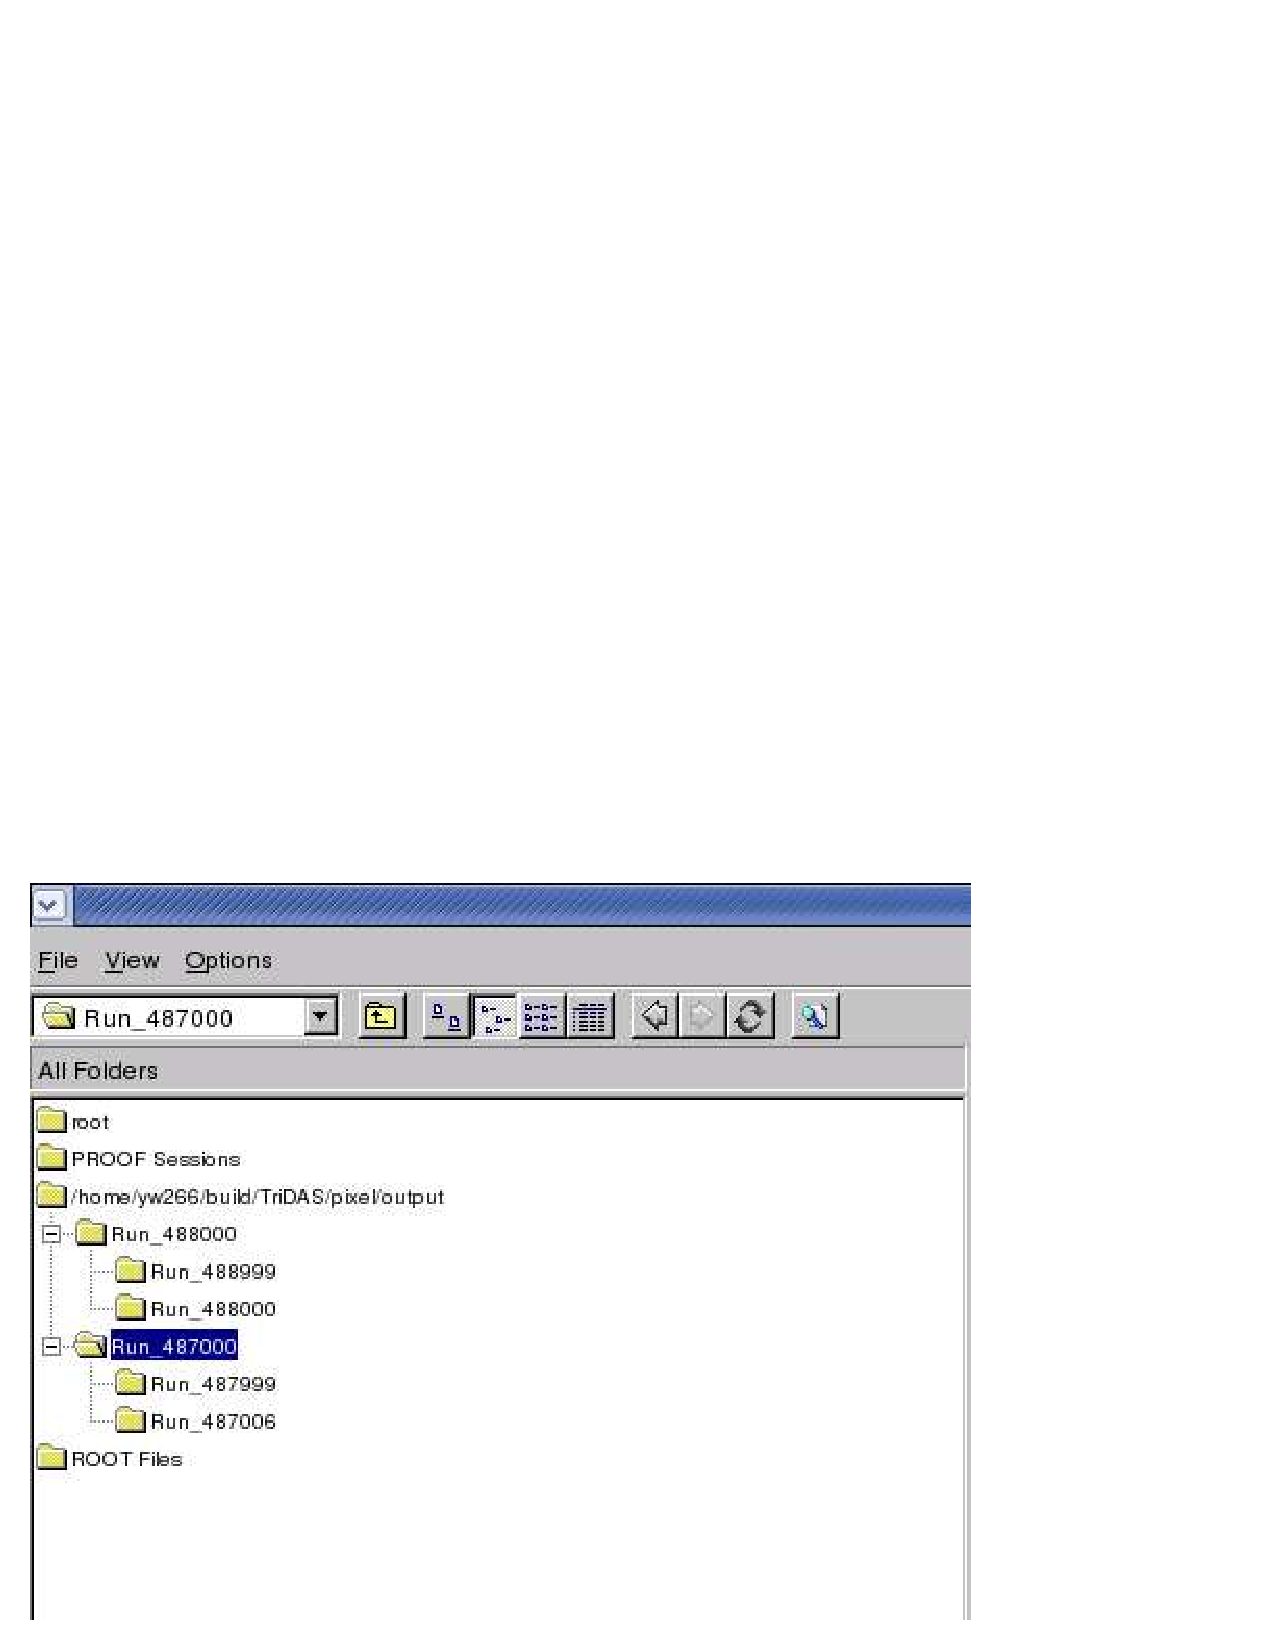
\includegraphics[width=7.5cm]{directory.pdf}
\caption{Output directory structure veiwing by ROOT.}
\label{fig:directory}
\end{minipage}
\hspace{0.5cm}
\begin{minipage}[htbp]{0.57\linewidth}
\centering
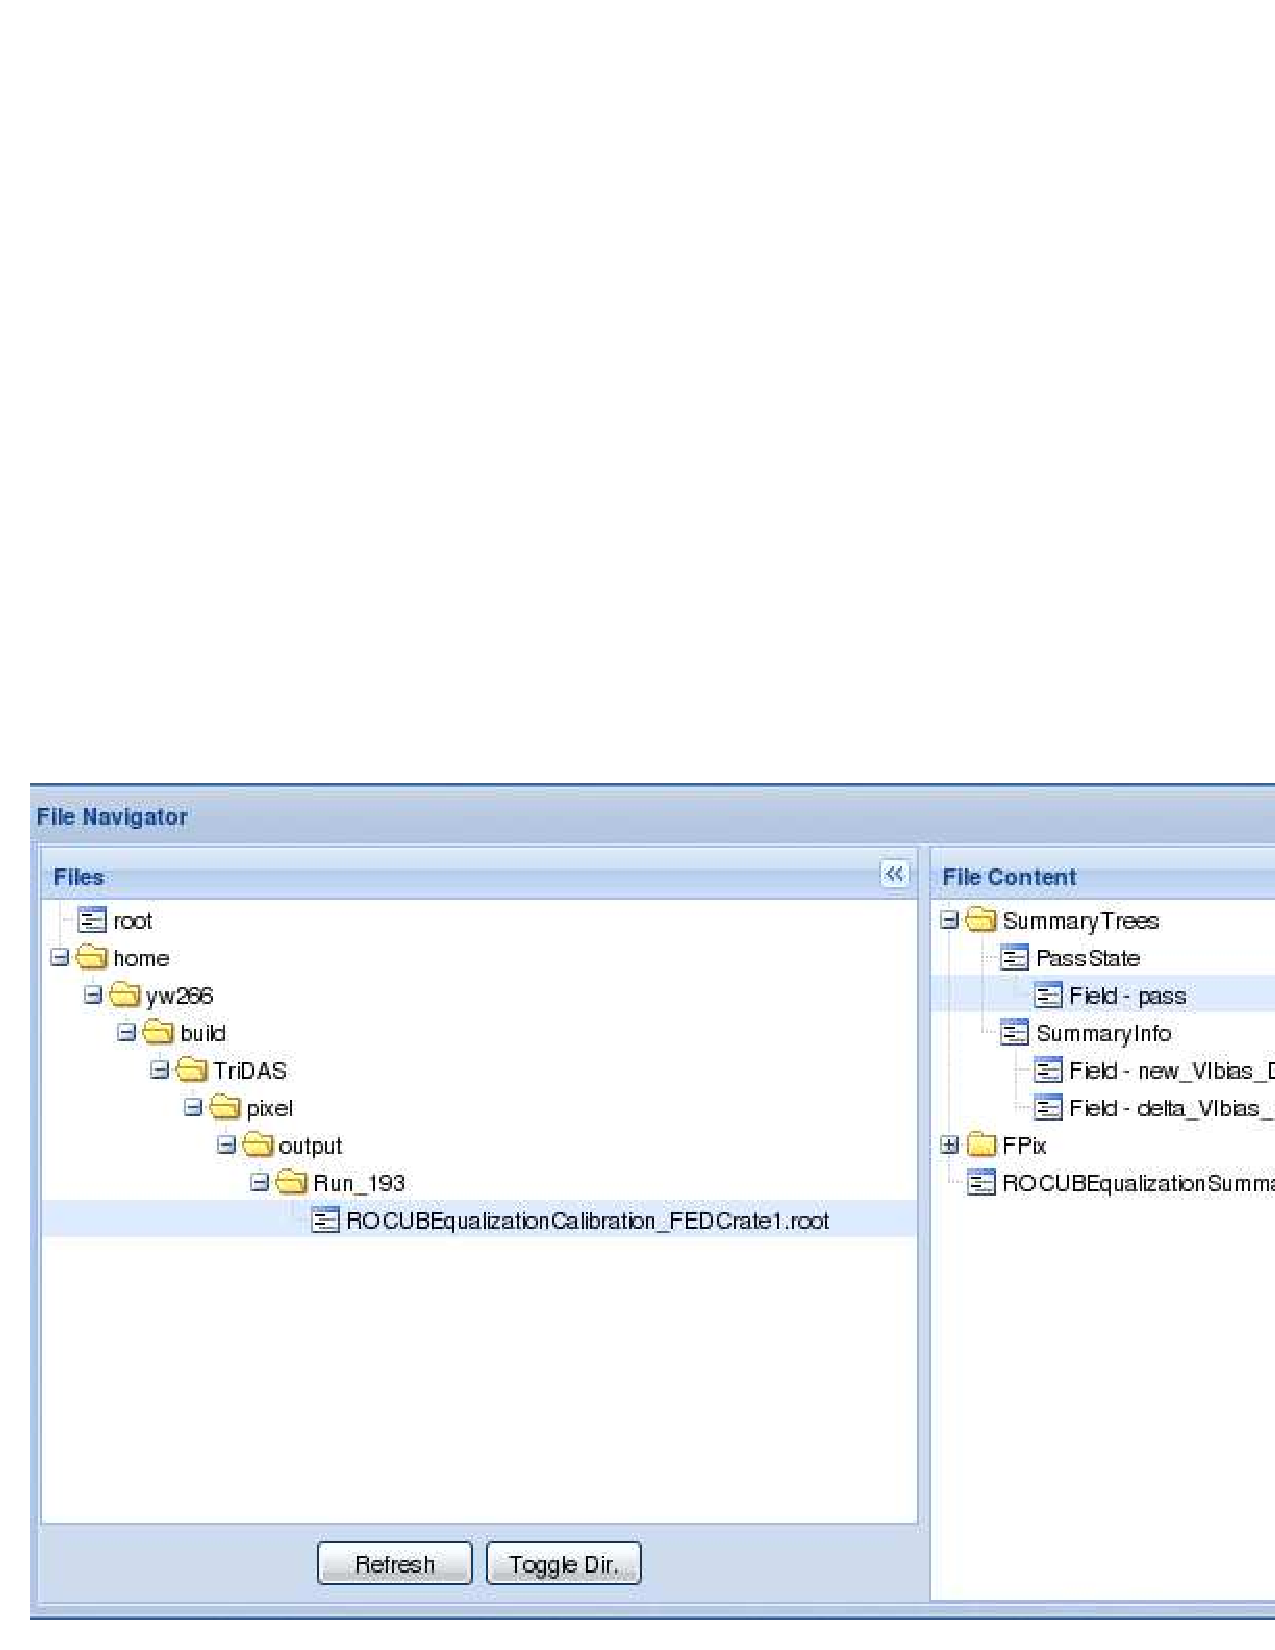
\includegraphics[width=9.5cm]{ROCUB_directory.pdf}
\caption{Output root directory structure veiwed by ROOT.}
\label{rootdirectory}
\end{minipage}
\end{figure}

\begin{figure}
\begin{minipage}[b]{0.47\linewidth} % A minipage that covers half the
\centering
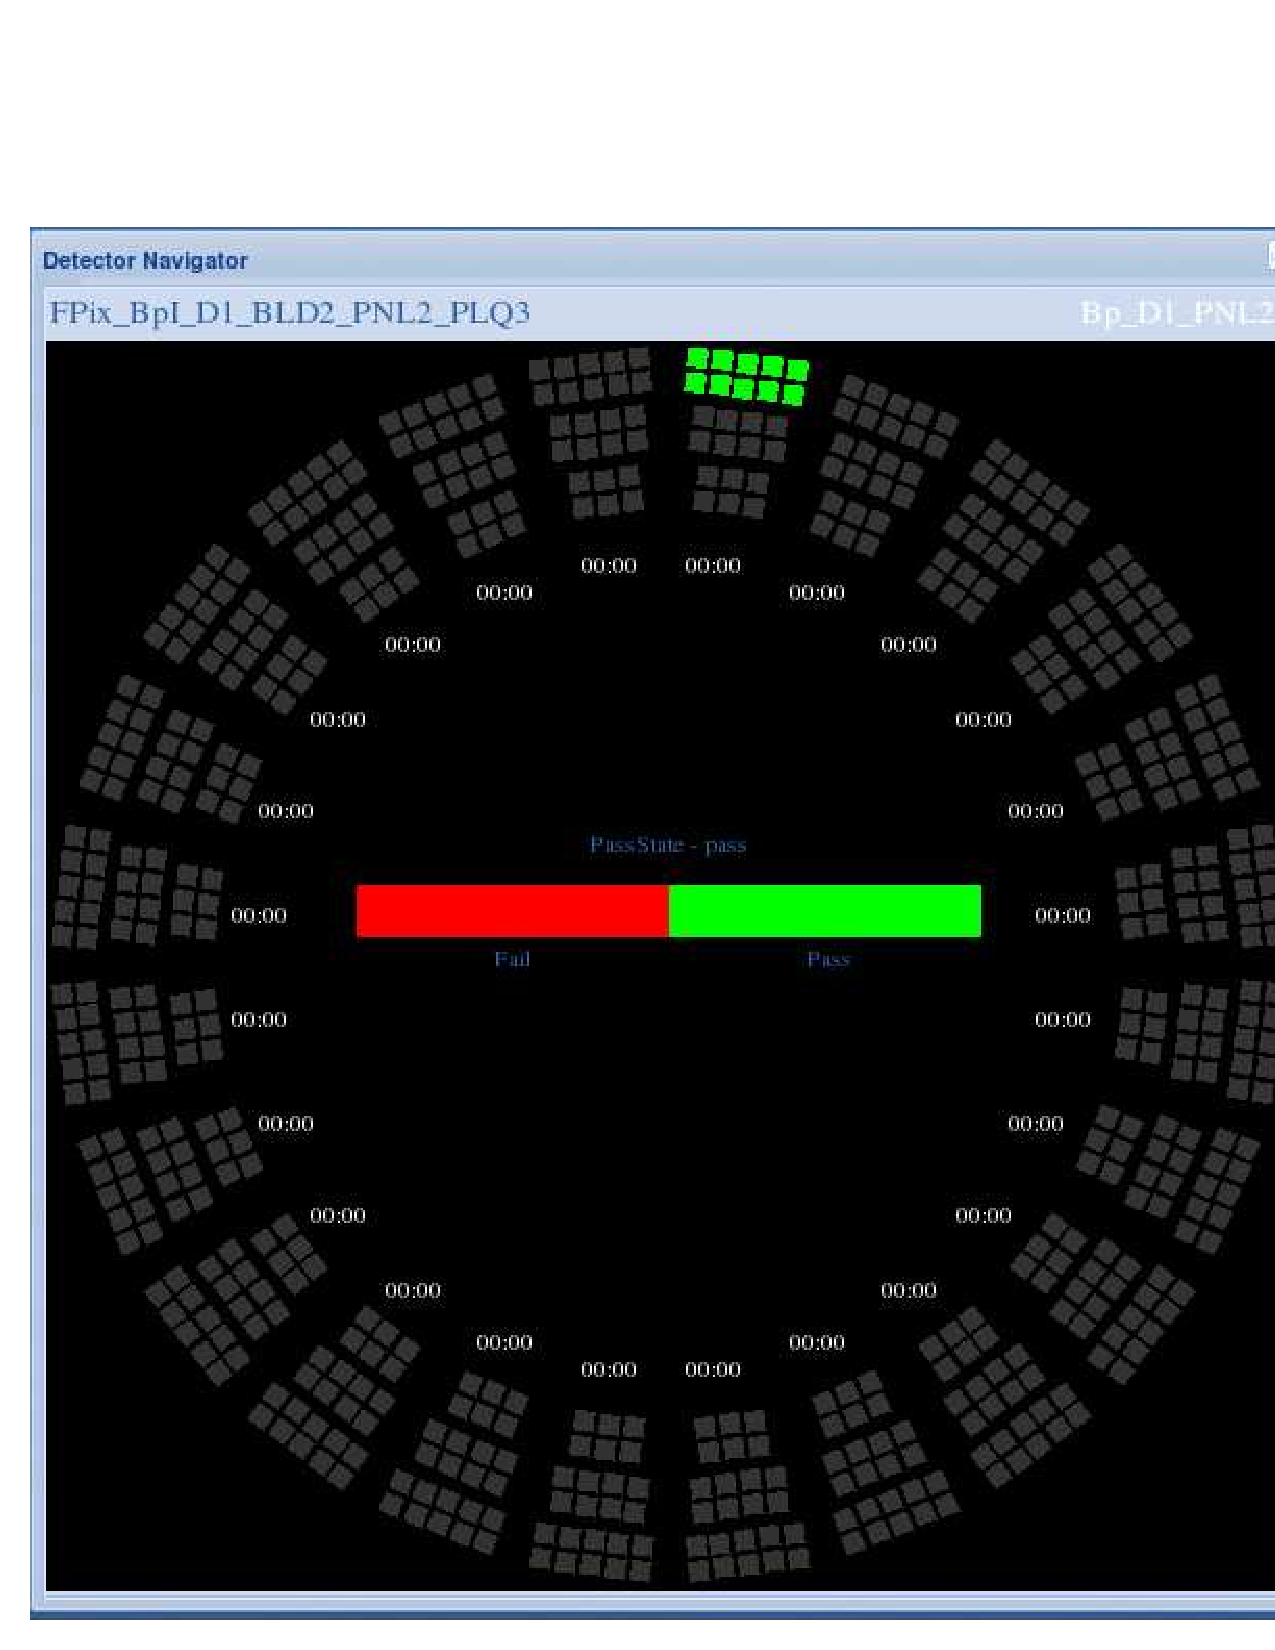
\includegraphics[width=5.5cm]{ROCUB_pass.pdf}
\caption{Pass information of ROCUBEqualization calibration viewed by histoviewer.}
\label{passinfo}
\end{minipage}
\hspace{0.5cm}
\begin{minipage}[b]{0.47\linewidth}
\centering
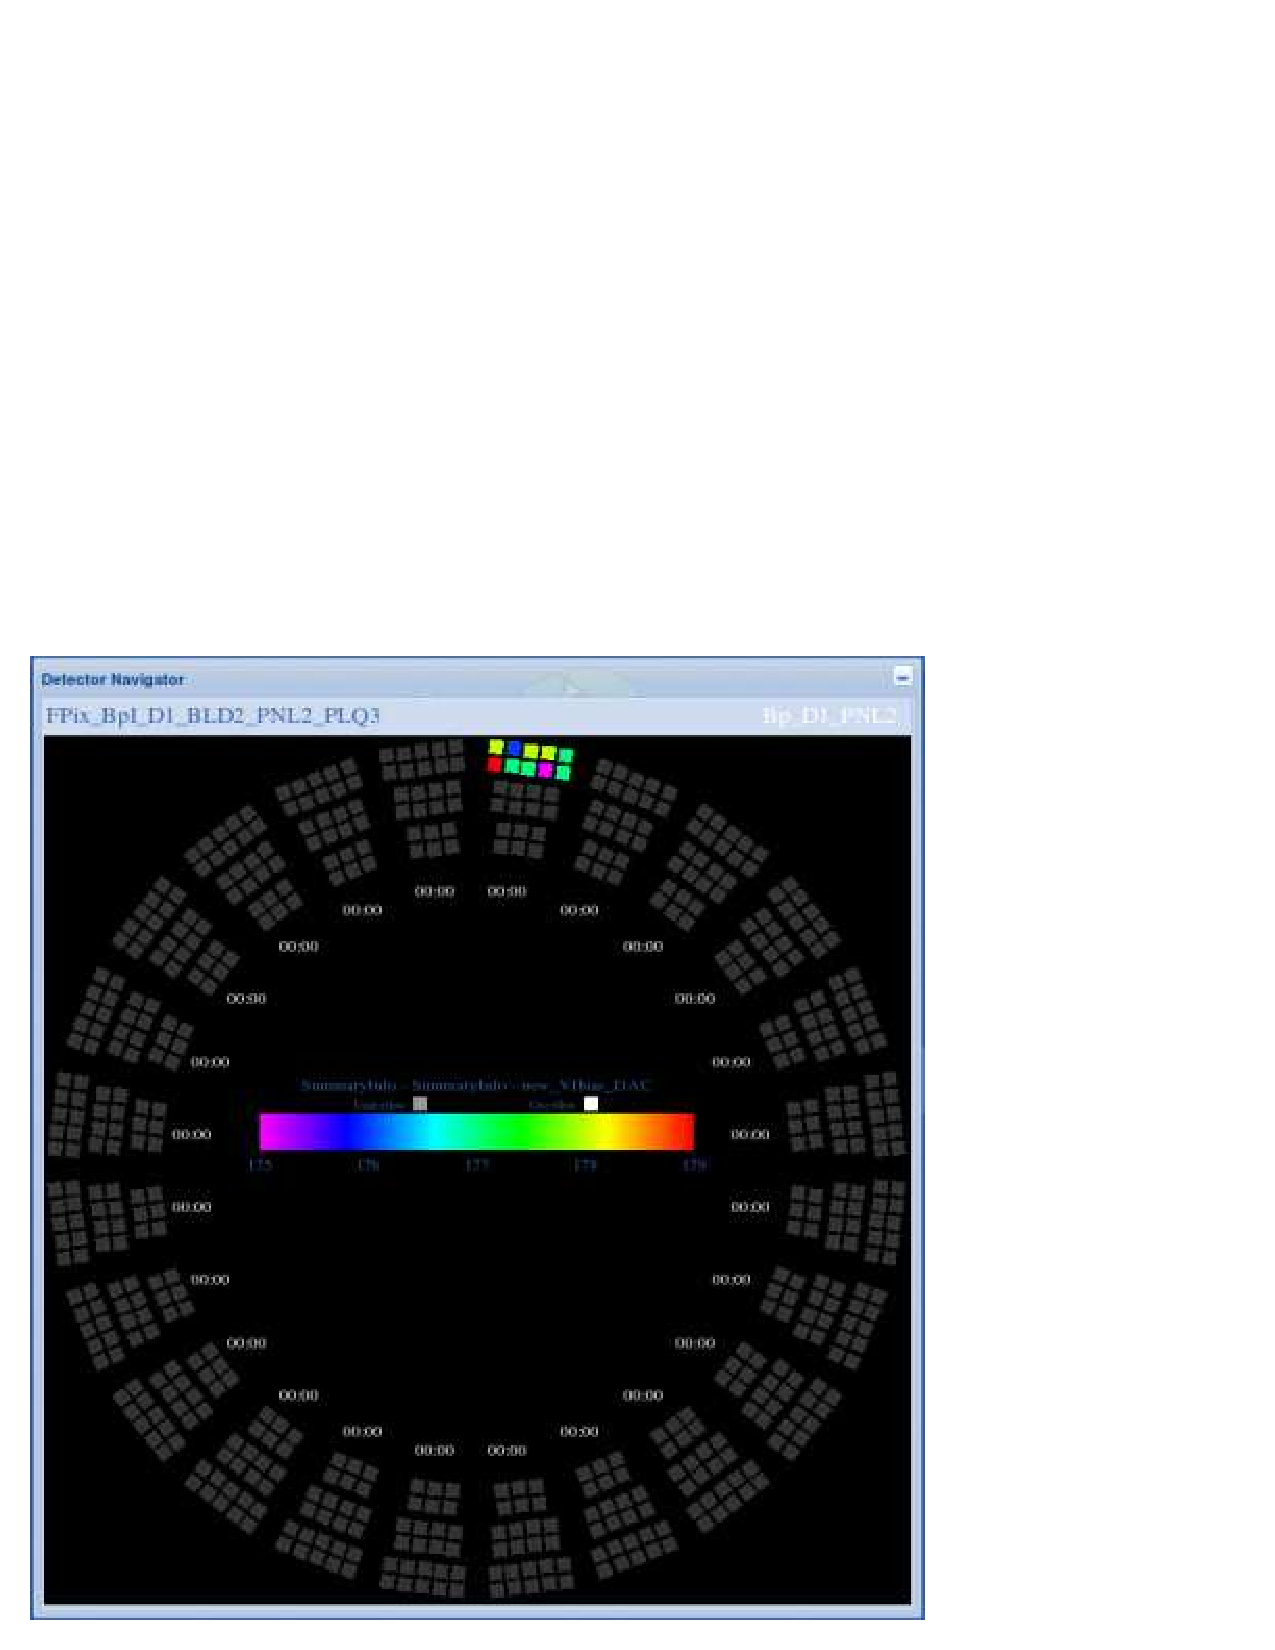
\includegraphics[width=8.5cm]{ROCUB_new_histoviewer.pdf}
\caption{New VIBias of ROCUBEqualization calibration veiwed by histoviewer.}
\label{summaryinfo}
\end{minipage}
\end{figure}

